% Options for packages loaded elsewhere
\PassOptionsToPackage{unicode}{hyperref}
\PassOptionsToPackage{hyphens}{url}
\PassOptionsToPackage{dvipsnames,svgnames,x11names}{xcolor}
%
\documentclass[
  letterpaper,
  DIV=11,
  numbers=noendperiod]{scrartcl}

\usepackage{amsmath,amssymb}
\usepackage{iftex}
\ifPDFTeX
  \usepackage[T1]{fontenc}
  \usepackage[utf8]{inputenc}
  \usepackage{textcomp} % provide euro and other symbols
\else % if luatex or xetex
  \usepackage{unicode-math}
  \defaultfontfeatures{Scale=MatchLowercase}
  \defaultfontfeatures[\rmfamily]{Ligatures=TeX,Scale=1}
\fi
\usepackage{lmodern}
\ifPDFTeX\else  
    % xetex/luatex font selection
\fi
% Use upquote if available, for straight quotes in verbatim environments
\IfFileExists{upquote.sty}{\usepackage{upquote}}{}
\IfFileExists{microtype.sty}{% use microtype if available
  \usepackage[]{microtype}
  \UseMicrotypeSet[protrusion]{basicmath} % disable protrusion for tt fonts
}{}
\makeatletter
\@ifundefined{KOMAClassName}{% if non-KOMA class
  \IfFileExists{parskip.sty}{%
    \usepackage{parskip}
  }{% else
    \setlength{\parindent}{0pt}
    \setlength{\parskip}{6pt plus 2pt minus 1pt}}
}{% if KOMA class
  \KOMAoptions{parskip=half}}
\makeatother
\usepackage{xcolor}
\setlength{\emergencystretch}{3em} % prevent overfull lines
\setcounter{secnumdepth}{5}
% Make \paragraph and \subparagraph free-standing
\makeatletter
\ifx\paragraph\undefined\else
  \let\oldparagraph\paragraph
  \renewcommand{\paragraph}{
    \@ifstar
      \xxxParagraphStar
      \xxxParagraphNoStar
  }
  \newcommand{\xxxParagraphStar}[1]{\oldparagraph*{#1}\mbox{}}
  \newcommand{\xxxParagraphNoStar}[1]{\oldparagraph{#1}\mbox{}}
\fi
\ifx\subparagraph\undefined\else
  \let\oldsubparagraph\subparagraph
  \renewcommand{\subparagraph}{
    \@ifstar
      \xxxSubParagraphStar
      \xxxSubParagraphNoStar
  }
  \newcommand{\xxxSubParagraphStar}[1]{\oldsubparagraph*{#1}\mbox{}}
  \newcommand{\xxxSubParagraphNoStar}[1]{\oldsubparagraph{#1}\mbox{}}
\fi
\makeatother

\usepackage{color}
\usepackage{fancyvrb}
\newcommand{\VerbBar}{|}
\newcommand{\VERB}{\Verb[commandchars=\\\{\}]}
\DefineVerbatimEnvironment{Highlighting}{Verbatim}{commandchars=\\\{\}}
% Add ',fontsize=\small' for more characters per line
\usepackage{framed}
\definecolor{shadecolor}{RGB}{241,243,245}
\newenvironment{Shaded}{\begin{snugshade}}{\end{snugshade}}
\newcommand{\AlertTok}[1]{\textcolor[rgb]{0.68,0.00,0.00}{#1}}
\newcommand{\AnnotationTok}[1]{\textcolor[rgb]{0.37,0.37,0.37}{#1}}
\newcommand{\AttributeTok}[1]{\textcolor[rgb]{0.40,0.45,0.13}{#1}}
\newcommand{\BaseNTok}[1]{\textcolor[rgb]{0.68,0.00,0.00}{#1}}
\newcommand{\BuiltInTok}[1]{\textcolor[rgb]{0.00,0.23,0.31}{#1}}
\newcommand{\CharTok}[1]{\textcolor[rgb]{0.13,0.47,0.30}{#1}}
\newcommand{\CommentTok}[1]{\textcolor[rgb]{0.37,0.37,0.37}{#1}}
\newcommand{\CommentVarTok}[1]{\textcolor[rgb]{0.37,0.37,0.37}{\textit{#1}}}
\newcommand{\ConstantTok}[1]{\textcolor[rgb]{0.56,0.35,0.01}{#1}}
\newcommand{\ControlFlowTok}[1]{\textcolor[rgb]{0.00,0.23,0.31}{\textbf{#1}}}
\newcommand{\DataTypeTok}[1]{\textcolor[rgb]{0.68,0.00,0.00}{#1}}
\newcommand{\DecValTok}[1]{\textcolor[rgb]{0.68,0.00,0.00}{#1}}
\newcommand{\DocumentationTok}[1]{\textcolor[rgb]{0.37,0.37,0.37}{\textit{#1}}}
\newcommand{\ErrorTok}[1]{\textcolor[rgb]{0.68,0.00,0.00}{#1}}
\newcommand{\ExtensionTok}[1]{\textcolor[rgb]{0.00,0.23,0.31}{#1}}
\newcommand{\FloatTok}[1]{\textcolor[rgb]{0.68,0.00,0.00}{#1}}
\newcommand{\FunctionTok}[1]{\textcolor[rgb]{0.28,0.35,0.67}{#1}}
\newcommand{\ImportTok}[1]{\textcolor[rgb]{0.00,0.46,0.62}{#1}}
\newcommand{\InformationTok}[1]{\textcolor[rgb]{0.37,0.37,0.37}{#1}}
\newcommand{\KeywordTok}[1]{\textcolor[rgb]{0.00,0.23,0.31}{\textbf{#1}}}
\newcommand{\NormalTok}[1]{\textcolor[rgb]{0.00,0.23,0.31}{#1}}
\newcommand{\OperatorTok}[1]{\textcolor[rgb]{0.37,0.37,0.37}{#1}}
\newcommand{\OtherTok}[1]{\textcolor[rgb]{0.00,0.23,0.31}{#1}}
\newcommand{\PreprocessorTok}[1]{\textcolor[rgb]{0.68,0.00,0.00}{#1}}
\newcommand{\RegionMarkerTok}[1]{\textcolor[rgb]{0.00,0.23,0.31}{#1}}
\newcommand{\SpecialCharTok}[1]{\textcolor[rgb]{0.37,0.37,0.37}{#1}}
\newcommand{\SpecialStringTok}[1]{\textcolor[rgb]{0.13,0.47,0.30}{#1}}
\newcommand{\StringTok}[1]{\textcolor[rgb]{0.13,0.47,0.30}{#1}}
\newcommand{\VariableTok}[1]{\textcolor[rgb]{0.07,0.07,0.07}{#1}}
\newcommand{\VerbatimStringTok}[1]{\textcolor[rgb]{0.13,0.47,0.30}{#1}}
\newcommand{\WarningTok}[1]{\textcolor[rgb]{0.37,0.37,0.37}{\textit{#1}}}

\providecommand{\tightlist}{%
  \setlength{\itemsep}{0pt}\setlength{\parskip}{0pt}}\usepackage{longtable,booktabs,array}
\usepackage{calc} % for calculating minipage widths
% Correct order of tables after \paragraph or \subparagraph
\usepackage{etoolbox}
\makeatletter
\patchcmd\longtable{\par}{\if@noskipsec\mbox{}\fi\par}{}{}
\makeatother
% Allow footnotes in longtable head/foot
\IfFileExists{footnotehyper.sty}{\usepackage{footnotehyper}}{\usepackage{footnote}}
\makesavenoteenv{longtable}
\usepackage{graphicx}
\makeatletter
\def\maxwidth{\ifdim\Gin@nat@width>\linewidth\linewidth\else\Gin@nat@width\fi}
\def\maxheight{\ifdim\Gin@nat@height>\textheight\textheight\else\Gin@nat@height\fi}
\makeatother
% Scale images if necessary, so that they will not overflow the page
% margins by default, and it is still possible to overwrite the defaults
% using explicit options in \includegraphics[width, height, ...]{}
\setkeys{Gin}{width=\maxwidth,height=\maxheight,keepaspectratio}
% Set default figure placement to htbp
\makeatletter
\def\fps@figure{htbp}
\makeatother
% definitions for citeproc citations
\NewDocumentCommand\citeproctext{}{}
\NewDocumentCommand\citeproc{mm}{%
  \begingroup\def\citeproctext{#2}\cite{#1}\endgroup}
\makeatletter
 % allow citations to break across lines
 \let\@cite@ofmt\@firstofone
 % avoid brackets around text for \cite:
 \def\@biblabel#1{}
 \def\@cite#1#2{{#1\if@tempswa , #2\fi}}
\makeatother
\newlength{\cslhangindent}
\setlength{\cslhangindent}{1.5em}
\newlength{\csllabelwidth}
\setlength{\csllabelwidth}{3em}
\newenvironment{CSLReferences}[2] % #1 hanging-indent, #2 entry-spacing
 {\begin{list}{}{%
  \setlength{\itemindent}{0pt}
  \setlength{\leftmargin}{0pt}
  \setlength{\parsep}{0pt}
  % turn on hanging indent if param 1 is 1
  \ifodd #1
   \setlength{\leftmargin}{\cslhangindent}
   \setlength{\itemindent}{-1\cslhangindent}
  \fi
  % set entry spacing
  \setlength{\itemsep}{#2\baselineskip}}}
 {\end{list}}
\usepackage{calc}
\newcommand{\CSLBlock}[1]{\hfill\break\parbox[t]{\linewidth}{\strut\ignorespaces#1\strut}}
\newcommand{\CSLLeftMargin}[1]{\parbox[t]{\csllabelwidth}{\strut#1\strut}}
\newcommand{\CSLRightInline}[1]{\parbox[t]{\linewidth - \csllabelwidth}{\strut#1\strut}}
\newcommand{\CSLIndent}[1]{\hspace{\cslhangindent}#1}

\KOMAoption{captions}{tableheading}
\makeatletter
\@ifpackageloaded{tcolorbox}{}{\usepackage[skins,breakable]{tcolorbox}}
\@ifpackageloaded{fontawesome5}{}{\usepackage{fontawesome5}}
\definecolor{quarto-callout-color}{HTML}{909090}
\definecolor{quarto-callout-note-color}{HTML}{0758E5}
\definecolor{quarto-callout-important-color}{HTML}{CC1914}
\definecolor{quarto-callout-warning-color}{HTML}{EB9113}
\definecolor{quarto-callout-tip-color}{HTML}{00A047}
\definecolor{quarto-callout-caution-color}{HTML}{FC5300}
\definecolor{quarto-callout-color-frame}{HTML}{acacac}
\definecolor{quarto-callout-note-color-frame}{HTML}{4582ec}
\definecolor{quarto-callout-important-color-frame}{HTML}{d9534f}
\definecolor{quarto-callout-warning-color-frame}{HTML}{f0ad4e}
\definecolor{quarto-callout-tip-color-frame}{HTML}{02b875}
\definecolor{quarto-callout-caution-color-frame}{HTML}{fd7e14}
\makeatother
\makeatletter
\@ifpackageloaded{caption}{}{\usepackage{caption}}
\AtBeginDocument{%
\ifdefined\contentsname
  \renewcommand*\contentsname{Table of contents}
\else
  \newcommand\contentsname{Table of contents}
\fi
\ifdefined\listfigurename
  \renewcommand*\listfigurename{List of Figures}
\else
  \newcommand\listfigurename{List of Figures}
\fi
\ifdefined\listtablename
  \renewcommand*\listtablename{List of Tables}
\else
  \newcommand\listtablename{List of Tables}
\fi
\ifdefined\figurename
  \renewcommand*\figurename{Figure}
\else
  \newcommand\figurename{Figure}
\fi
\ifdefined\tablename
  \renewcommand*\tablename{Table}
\else
  \newcommand\tablename{Table}
\fi
}
\@ifpackageloaded{float}{}{\usepackage{float}}
\floatstyle{ruled}
\@ifundefined{c@chapter}{\newfloat{codelisting}{h}{lop}}{\newfloat{codelisting}{h}{lop}[chapter]}
\floatname{codelisting}{Listing}
\newcommand*\listoflistings{\listof{codelisting}{List of Listings}}
\makeatother
\makeatletter
\makeatother
\makeatletter
\@ifpackageloaded{caption}{}{\usepackage{caption}}
\@ifpackageloaded{subcaption}{}{\usepackage{subcaption}}
\makeatother

\ifLuaTeX
  \usepackage{selnolig}  % disable illegal ligatures
\fi
\usepackage{bookmark}

\IfFileExists{xurl.sty}{\usepackage{xurl}}{} % add URL line breaks if available
\urlstyle{same} % disable monospaced font for URLs
\hypersetup{
  pdftitle={Forest manipulation experiment reveals divergent controls on the sources and age of lateral DOC and CO₂ export},
  pdfauthor={Audrey Campeau; A. Zannella and M. Wallin},
  colorlinks=true,
  linkcolor={blue},
  filecolor={Maroon},
  citecolor={Blue},
  urlcolor={Blue},
  pdfcreator={LaTeX via pandoc}}


\title{Forest manipulation experiment reveals divergent controls on the
sources and age of lateral DOC and CO₂ export}
\author{Audrey Campeau \and A. Zannella and M. Wallin}
\date{2025-08-21}

\begin{document}
\maketitle

\renewcommand*\contentsname{Table of contents}
{
\hypersetup{linkcolor=}
\setcounter{tocdepth}{2}
\tableofcontents
}

\section{Introduction}\label{introduction}

\subsection{General Context}\label{general-context}

\begin{itemize}
\item
  Lateral C export is a significant fraction of watershed C balance.
\item
  Forested catchments contain a large OM storage (Ledesma et al. 2013)
\item
  LCE and NEE are connected over long timescale, by hydrology (Öquist et
  al. 2014)
\end{itemize}

\subsection{Research Question}\label{research-question}

What are the controls over the sources and age of lateral CO2 and DOC
export in forested catchments? Can a forest manipulation experiment
(forest clearcut and ditch cleaning) inform us on the controls of these
C sources?

\subsection{Hypothesis}\label{hypothesis}

The CO2 source and age is more closely linked to the forest C sink (A.
Campeau et al. 2019), so clearcutting the forest should have an impact
on C sources and age

The DOC source and age is linked to discharge (Audrey Campeau et al.
2017) or water table position (A. Campeau et al. 2019), so changes in
watershed hydrology, caused by clear-cutting and draining, should change
the source and age of DOC.

\subsection{Main Conclusion}\label{main-conclusion}

DOC is controled more by \emph{hydrological processes}, which determines
what material is being mobilised, while CO2 is controled more by
\emph{biological processes,} which fuels CO2 in the watershed. Both are
therefore controled by different processes, but will likely respond to
changes in climate, albeit via different drivers.

\section{Methodology}\label{methodology}

\subsection{Study Site and Treatment:}\label{study-site-and-treatment}

\begin{itemize}
\item
  Six headwater catchments are included in this study:

  \begin{itemize}
  \item
    2 pristine sites (C1 and C2)
  \item
    4 treated watersheds (DC1 to DC4).
  \end{itemize}
\item
  The DC sites received different treatments:

  \begin{itemize}
  \item
    Forest in all four sites was clearcut - around July 2020.
  \item
    Two sites, DC1 and DC3, were also ditch cleaned - in September 2021.
  \item
    The treatments are named as follow (pristine, clear-cut and ditch
    cleaning)
  \end{itemize}
\end{itemize}

\subsection{Map of the study sites (draw schematic
instead)}\label{map-of-the-study-sites-draw-schematic-instead}

\begin{figure}[H]

{\centering \includegraphics{Trollberget_All infrastructure_plusPlanned_aerial_dc catchments.jpg}

}

\caption{Map of the infrastructure and catchment delineation for each
site in the Trollberget ExperimentalArea}

\end{figure}%

\subsection{Field measurements:}\label{field-measurements}

\begin{itemize}
\item
  All four sites are monitored for flow and water chemistry on a near
  continuous basis.
\item
  Radiocarbon and stable C isotope measurements were collected at those
  six sites simultaniously and throughout various treatment stages.
\item
  14C measurements

  \begin{itemize}
  \item
    Start 2020-03-12
  \item
    End 2022-10-25
  \end{itemize}
\end{itemize}

\section{Results}\label{results}

\subsection{Hydrographs and carbon
concentrations}\label{hydrographs-and-carbon-concentrations}

\begin{Shaded}
\begin{Highlighting}[]
\CommentTok{\# Define operation periods for treatments::::::::::::::::::::::::::::::::::::::::::}
  
\NormalTok{clearcut\_start }\OtherTok{\textless{}{-}} \FunctionTok{as.Date}\NormalTok{(}\StringTok{"2020{-}07{-}01"}\NormalTok{)}
\NormalTok{clearcut\_end }\OtherTok{\textless{}{-}} \FunctionTok{as.Date}\NormalTok{(}\StringTok{"2020{-}08{-}25"}\NormalTok{)}
\NormalTok{ditch\_cleaning\_start }\OtherTok{\textless{}{-}} \FunctionTok{as.Date}\NormalTok{(}\StringTok{"2021{-}09{-}01"}\NormalTok{)}
\NormalTok{ditch\_cleaning\_end }\OtherTok{\textless{}{-}} \FunctionTok{as.Date}\NormalTok{(}\StringTok{"2021{-}09{-}30"}\NormalTok{)}

 
\CommentTok{\# Make the precipitation graph :::::::::::::::::::::::::::::::::::::::::::::::::::::}


\NormalTok{precipitation}\OtherTok{=} \FunctionTok{ggplot}\NormalTok{(DC\_Q }\SpecialCharTok{\%\textgreater{}\%}
         \FunctionTok{filter}\NormalTok{(Site\_id }\SpecialCharTok{\%in\%} \FunctionTok{c}\NormalTok{(}\StringTok{"DC1"}\NormalTok{)),}
       \FunctionTok{aes}\NormalTok{(}\AttributeTok{y =}\NormalTok{ P, }\AttributeTok{x =} \FunctionTok{as.Date}\NormalTok{(Date), }\AttributeTok{color =}\NormalTok{ Site\_id)) }\SpecialCharTok{+}
  
  \CommentTok{\# Add gray background bars for operations}
  \FunctionTok{annotate}\NormalTok{(}\StringTok{"rect"}\NormalTok{, }
           \AttributeTok{xmin =}\NormalTok{ clearcut\_start, }\AttributeTok{xmax =}\NormalTok{ clearcut\_end,}
           \AttributeTok{ymin =} \SpecialCharTok{{-}}\ConstantTok{Inf}\NormalTok{, }\AttributeTok{ymax =} \ConstantTok{Inf}\NormalTok{, }\AttributeTok{fill =} \StringTok{"gray70"}\NormalTok{, }\AttributeTok{alpha =} \FloatTok{0.3}\NormalTok{) }\SpecialCharTok{+}
  
  \FunctionTok{annotate}\NormalTok{(}\StringTok{"rect"}\NormalTok{, }
           \AttributeTok{xmin =}\NormalTok{ ditch\_cleaning\_start, }\AttributeTok{xmax =}\NormalTok{ ditch\_cleaning\_end,}
           \AttributeTok{ymin =} \SpecialCharTok{{-}}\ConstantTok{Inf}\NormalTok{, }\AttributeTok{ymax =} \ConstantTok{Inf}\NormalTok{, }\AttributeTok{fill =} \StringTok{"gray70"}\NormalTok{, }\AttributeTok{alpha =} \FloatTok{0.3}\NormalTok{) }\SpecialCharTok{+}
  
  \FunctionTok{geom\_bar}\NormalTok{(}\AttributeTok{stat =} \StringTok{\textquotesingle{}identity\textquotesingle{}}\NormalTok{, }\AttributeTok{width=}\FloatTok{0.2}\NormalTok{) }\SpecialCharTok{+}
  \FunctionTok{labs}\NormalTok{( }\AttributeTok{y=} \StringTok{"Precipitation (mm/day)"}\NormalTok{) }\SpecialCharTok{+}
  \FunctionTok{scale\_y\_reverse}\NormalTok{()}\SpecialCharTok{+}
  \FunctionTok{scale\_color\_manual}\NormalTok{(}\AttributeTok{values=}\NormalTok{site\_colors\_6)}\SpecialCharTok{+} \CommentTok{\#"}
  \FunctionTok{scale\_x\_date}\NormalTok{(}\AttributeTok{limits=}\FunctionTok{c}\NormalTok{(}\FunctionTok{as.Date}\NormalTok{(}\StringTok{"2020{-}01{-}01"}\NormalTok{), }\FunctionTok{as.Date}\NormalTok{(}\StringTok{"2022{-}11{-}01"}\NormalTok{)),}
               \AttributeTok{date\_labels =} \StringTok{"\%b{-}\%Y"}\NormalTok{, }\AttributeTok{date\_breaks =} \StringTok{"6 months"}\NormalTok{) }\SpecialCharTok{+}
  
  
  \FunctionTok{labs}\NormalTok{(}\AttributeTok{y =} \StringTok{"P (mm/d)"}\NormalTok{,  }\AttributeTok{x =} \StringTok{"Date"}\NormalTok{) }\SpecialCharTok{+}
  \FunctionTok{theme}\NormalTok{(}\AttributeTok{legend.position =} \StringTok{"none"}\NormalTok{, }\AttributeTok{axis.title.x =} \FunctionTok{element\_blank}\NormalTok{())}



\CommentTok{\# Make Hydrograph :::::::::::::::::::::::::::::::::::::::::::::::::::::}

\NormalTok{hydrograph}\OtherTok{=} \FunctionTok{ggplot}\NormalTok{(DC\_Q }\SpecialCharTok{\%\textgreater{}\%}
         \FunctionTok{filter}\NormalTok{(Site\_id }\SpecialCharTok{\%in\%} \FunctionTok{c}\NormalTok{(}\StringTok{"DC2"}\NormalTok{, }\StringTok{"DC3"}\NormalTok{)),}
       \FunctionTok{aes}\NormalTok{(}\AttributeTok{y =}\NormalTok{ q\_md}\SpecialCharTok{*}\DecValTok{1000}\NormalTok{, }\AttributeTok{x =} \FunctionTok{as.Date}\NormalTok{(Date), }\AttributeTok{color =}\NormalTok{ Site\_id)) }\SpecialCharTok{+}
  
  \CommentTok{\# Add gray background bars for operations}
  \FunctionTok{annotate}\NormalTok{(}\StringTok{"rect"}\NormalTok{, }
           \AttributeTok{xmin =}\NormalTok{ clearcut\_start, }\AttributeTok{xmax =}\NormalTok{ clearcut\_end,}
           \AttributeTok{ymin =} \SpecialCharTok{{-}}\ConstantTok{Inf}\NormalTok{, }\AttributeTok{ymax =} \ConstantTok{Inf}\NormalTok{,}
           \AttributeTok{fill =} \StringTok{"gray70"}\NormalTok{, }\AttributeTok{alpha =} \FloatTok{0.3}\NormalTok{) }\SpecialCharTok{+}
  
  \FunctionTok{annotate}\NormalTok{(}\StringTok{"rect"}\NormalTok{, }
           \AttributeTok{xmin =}\NormalTok{ ditch\_cleaning\_start, }\AttributeTok{xmax =}\NormalTok{ ditch\_cleaning\_end,}
           \AttributeTok{ymin =} \SpecialCharTok{{-}}\ConstantTok{Inf}\NormalTok{, }\AttributeTok{ymax =} \ConstantTok{Inf}\NormalTok{,}
           \AttributeTok{fill =} \StringTok{"gray70"}\NormalTok{, }\AttributeTok{alpha =} \FloatTok{0.3}\NormalTok{) }\SpecialCharTok{+}
  
  \CommentTok{\# Add the discharge lines}
  \FunctionTok{geom\_line}\NormalTok{() }\SpecialCharTok{+}
  \FunctionTok{scale\_color\_manual}\NormalTok{(}\AttributeTok{values=}\NormalTok{site\_colors\_6)}\SpecialCharTok{+} \CommentTok{\#"}
   
  \CommentTok{\# Add text labels for operations}
 \FunctionTok{annotate}\NormalTok{(}\StringTok{"text"}\NormalTok{, }\AttributeTok{x =}\NormalTok{ clearcut\_start }\SpecialCharTok{+}\NormalTok{ (clearcut\_end }\SpecialCharTok{{-}}\NormalTok{ clearcut\_start)}\SpecialCharTok{/}\DecValTok{2}\NormalTok{, }\AttributeTok{y =} \ConstantTok{Inf}\NormalTok{, }
           \AttributeTok{label =} \StringTok{"Forest clear cut operations}\SpecialCharTok{\textbackslash{}n}\StringTok{(July 2020)"}\NormalTok{,}
           \AttributeTok{vjust =} \FloatTok{1.2}\NormalTok{, }\AttributeTok{hjust =} \FloatTok{0.5}\NormalTok{, }\AttributeTok{size =} \FloatTok{3.5}\NormalTok{, }\AttributeTok{color =} \StringTok{"black"}\NormalTok{) }\SpecialCharTok{+}
  
  \FunctionTok{annotate}\NormalTok{(}\StringTok{"text"}\NormalTok{, }\AttributeTok{x =}\NormalTok{ ditch\_cleaning\_start }\SpecialCharTok{+}\NormalTok{ (ditch\_cleaning\_end }\SpecialCharTok{{-}}\NormalTok{    ditch\_cleaning\_start)}\SpecialCharTok{/}\DecValTok{2}\NormalTok{, }\AttributeTok{y =} \ConstantTok{Inf}\NormalTok{, }
           \AttributeTok{label =} \StringTok{"Ditch cleaning operations}\SpecialCharTok{\textbackslash{}n}\StringTok{(September 2021)"}\NormalTok{,}
           \AttributeTok{vjust =} \FloatTok{1.2}\NormalTok{, }\AttributeTok{hjust =} \FloatTok{0.5}\NormalTok{, }\AttributeTok{size =} \FloatTok{3.5}\NormalTok{, }\AttributeTok{color =} \StringTok{"black"}\NormalTok{) }\SpecialCharTok{+}
  
  \FunctionTok{scale\_x\_date}\NormalTok{(}\AttributeTok{limits=}\FunctionTok{c}\NormalTok{(}\FunctionTok{as.Date}\NormalTok{(}\StringTok{"2020{-}01{-}01"}\NormalTok{), }\FunctionTok{as.Date}\NormalTok{(}\StringTok{"2022{-}11{-}01"}\NormalTok{)),}
                 \AttributeTok{date\_labels =} \StringTok{"\%b{-}\%Y"}\NormalTok{, }\AttributeTok{date\_breaks =} \StringTok{"6 months"}\NormalTok{) }\SpecialCharTok{+}
  \FunctionTok{labs}\NormalTok{(}\AttributeTok{y =} \StringTok{"q (mm/d)"}\NormalTok{,   }\AttributeTok{x =} \StringTok{"Date"}\NormalTok{,  }\AttributeTok{color =} \StringTok{"Stream"}\NormalTok{) }\SpecialCharTok{+}
  \FunctionTok{theme}\NormalTok{(}\AttributeTok{legend.position =} \StringTok{"none"}\NormalTok{, }\AttributeTok{axis.title.x =} \FunctionTok{element\_blank}\NormalTok{())}



\FunctionTok{ggarrange}\NormalTok{(precipitation, hydrograph,}
          \AttributeTok{ncol=}\DecValTok{1}\NormalTok{, }\AttributeTok{align=}\StringTok{"v"}\NormalTok{)}
\end{Highlighting}
\end{Shaded}

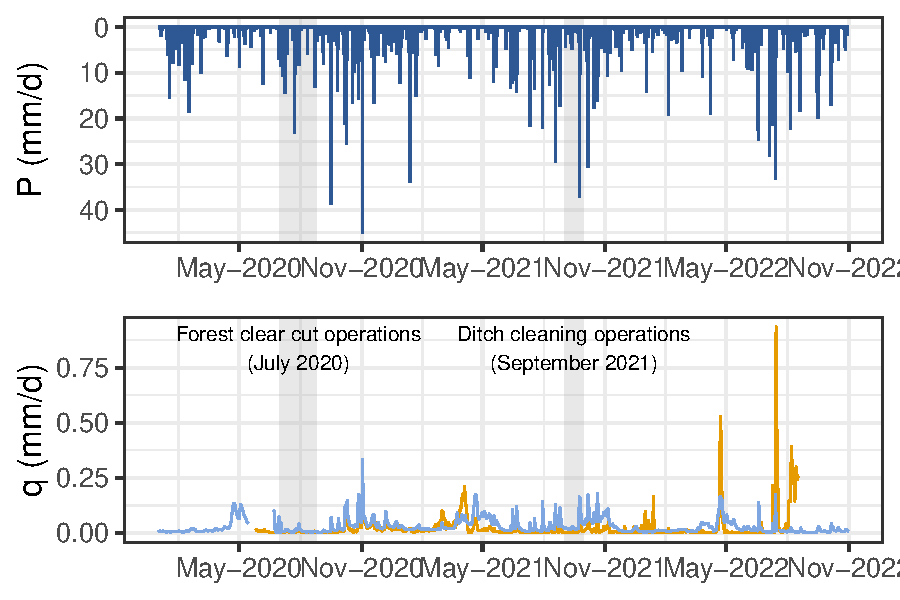
\includegraphics{index_files/figure-pdf/unnamed-chunk-2-1.pdf}

\begin{Shaded}
\begin{Highlighting}[]
\CommentTok{\# Timeseries 14C per site, CO2 and DOC seperately}
\NormalTok{plot\_timeseries }\OtherTok{=} \ControlFlowTok{function}\NormalTok{(data, y\_var,labs\_y) \{}
  \FunctionTok{ggplot}\NormalTok{(data, }\FunctionTok{aes}\NormalTok{(}\AttributeTok{x=}\NormalTok{Date, }\AttributeTok{y=}\SpecialCharTok{!!}\FunctionTok{sym}\NormalTok{(y\_var), }\AttributeTok{group=}\NormalTok{Site\_id, }\AttributeTok{color=}\NormalTok{Site\_id)) }\SpecialCharTok{+}
    \FunctionTok{geom\_line}\NormalTok{(}\AttributeTok{data=}\NormalTok{data[}\SpecialCharTok{!}\FunctionTok{is.na}\NormalTok{(data[[y\_var]]), ]) }\SpecialCharTok{+}
    \FunctionTok{geom\_point}\NormalTok{(}\AttributeTok{size=}\DecValTok{3}\NormalTok{) }\SpecialCharTok{+}
  
  \CommentTok{\# Add gray background bars for operations}
  \FunctionTok{annotate}\NormalTok{(}\StringTok{"rect"}\NormalTok{, }
           \AttributeTok{xmin =}\NormalTok{ clearcut\_start, }\AttributeTok{xmax =}\NormalTok{ clearcut\_end,}
           \AttributeTok{ymin =} \SpecialCharTok{{-}}\ConstantTok{Inf}\NormalTok{, }\AttributeTok{ymax =} \ConstantTok{Inf}\NormalTok{,}
           \AttributeTok{fill =} \StringTok{"gray70"}\NormalTok{, }\AttributeTok{alpha =} \FloatTok{0.3}\NormalTok{) }\SpecialCharTok{+}
  
  \FunctionTok{annotate}\NormalTok{(}\StringTok{"rect"}\NormalTok{, }
           \AttributeTok{xmin =}\NormalTok{ ditch\_cleaning\_start, }\AttributeTok{xmax =}\NormalTok{ ditch\_cleaning\_end,}
           \AttributeTok{ymin =} \SpecialCharTok{{-}}\ConstantTok{Inf}\NormalTok{, }\AttributeTok{ymax =} \ConstantTok{Inf}\NormalTok{,}
           \AttributeTok{fill =} \StringTok{"gray70"}\NormalTok{, }\AttributeTok{alpha =} \FloatTok{0.3}\NormalTok{) }\SpecialCharTok{+}
    
    \FunctionTok{scale\_x\_date}\NormalTok{(}\AttributeTok{limits=}\FunctionTok{c}\NormalTok{(}\FunctionTok{as.Date}\NormalTok{(}\StringTok{"2020{-}01{-}01"}\NormalTok{), }\FunctionTok{as.Date}\NormalTok{(}\StringTok{"2022{-}11{-}01"}\NormalTok{)),}
                 \AttributeTok{date\_labels =} \StringTok{"\%m{-}\%Y"}\NormalTok{, }\AttributeTok{date\_breaks =} \StringTok{"3 months"}\NormalTok{) }\SpecialCharTok{+}
    \FunctionTok{scale\_color\_manual}\NormalTok{(}\AttributeTok{values=}\FunctionTok{c}\NormalTok{(site\_colors\_6))}\SpecialCharTok{+}
    \FunctionTok{labs}\NormalTok{(}\AttributeTok{y=}\NormalTok{labs\_y)}\SpecialCharTok{+}
    
    \FunctionTok{theme}\NormalTok{( }\CommentTok{\# set margins to align combined plots }
      \AttributeTok{plot.margin =} \FunctionTok{margin}\NormalTok{(}\FloatTok{5.5}\NormalTok{, }\FloatTok{5.5}\NormalTok{, }\FloatTok{5.5}\NormalTok{, }\FloatTok{5.5}\NormalTok{, }\StringTok{"pt"}\NormalTok{),}
      \AttributeTok{axis.text.x =} \FunctionTok{element\_text}\NormalTok{(}\AttributeTok{size =} \DecValTok{10}\NormalTok{),}
      \AttributeTok{axis.title.x =} \FunctionTok{element\_text}\NormalTok{(}\AttributeTok{size =} \DecValTok{11}\NormalTok{),}
      \AttributeTok{panel.grid.major =} \FunctionTok{element\_line}\NormalTok{(}\AttributeTok{size =} \FloatTok{0.5}\NormalTok{),}
      \AttributeTok{panel.grid.minor =} \FunctionTok{element\_line}\NormalTok{(}\AttributeTok{size =} \FloatTok{0.25}\NormalTok{)}
\NormalTok{    )}

\NormalTok{\}}



\CommentTok{\#Concentration timeseries}
\NormalTok{timeserie\_14CDOC }\OtherTok{=}\NormalTok{ ggExtra}\SpecialCharTok{::}\FunctionTok{ggMarginal}\NormalTok{(}
  \FunctionTok{plot\_timeseries}\NormalTok{(DC\_Q, }\StringTok{"DOC\_14C\_Modern"}\NormalTok{, }\StringTok{"14C{-}DOC (\%)"}\NormalTok{)}\SpecialCharTok{+}
  \FunctionTok{scale\_y\_continuous}\NormalTok{(}\AttributeTok{limits=}\FunctionTok{c}\NormalTok{(}\DecValTok{95}\NormalTok{,}\DecValTok{115}\NormalTok{))}\SpecialCharTok{+}
  \FunctionTok{theme}\NormalTok{(}\AttributeTok{legend.position =} \StringTok{"none"}\NormalTok{, }\AttributeTok{axis.title.x =} \FunctionTok{element\_blank}\NormalTok{()),}
  \AttributeTok{margins=}\FunctionTok{c}\NormalTok{(}\StringTok{"y"}\NormalTok{), }\AttributeTok{type =} \StringTok{"boxplot"}\NormalTok{, }\AttributeTok{groupColour =} \ConstantTok{TRUE}\NormalTok{, }\AttributeTok{groupFill =} \ConstantTok{TRUE}\NormalTok{ )}


\NormalTok{timeserie\_DOC }\OtherTok{=}\NormalTok{ ggExtra}\SpecialCharTok{::}\FunctionTok{ggMarginal}\NormalTok{(}
  \FunctionTok{plot\_timeseries}\NormalTok{(DC\_Q, }\StringTok{"DOC\_mgL"}\NormalTok{, }\StringTok{"DOC (mg/L)"}\NormalTok{)}\SpecialCharTok{+}
  \FunctionTok{theme}\NormalTok{(}\AttributeTok{legend.position =} \StringTok{"top"}\NormalTok{, }\AttributeTok{axis.title.x =} \FunctionTok{element\_blank}\NormalTok{()),}
  \AttributeTok{margins=}\FunctionTok{c}\NormalTok{(}\StringTok{"y"}\NormalTok{), }\AttributeTok{type =} \StringTok{"boxplot"}\NormalTok{, }\AttributeTok{groupColour =} \ConstantTok{TRUE}\NormalTok{, }\AttributeTok{groupFill =} \ConstantTok{TRUE}\NormalTok{ )}


\NormalTok{timeserie\_14CCO2 }\OtherTok{=}\NormalTok{ ggExtra}\SpecialCharTok{::}\FunctionTok{ggMarginal}\NormalTok{(}
  \FunctionTok{plot\_timeseries}\NormalTok{(DC\_Q, }\StringTok{"CO2\_14C\_Modern"}\NormalTok{, }\StringTok{"14C{-}CO2 (\%)"}\NormalTok{)}\SpecialCharTok{+}
  \FunctionTok{scale\_y\_continuous}\NormalTok{(}\AttributeTok{limits=}\FunctionTok{c}\NormalTok{(}\DecValTok{95}\NormalTok{,}\DecValTok{115}\NormalTok{))}\SpecialCharTok{+}
   \FunctionTok{theme}\NormalTok{(}\AttributeTok{legend.position =} \StringTok{"none"}\NormalTok{, }\AttributeTok{axis.title.x =} \FunctionTok{element\_blank}\NormalTok{()),}
  \AttributeTok{margins=}\FunctionTok{c}\NormalTok{(}\StringTok{"y"}\NormalTok{), }\AttributeTok{type =} \StringTok{"boxplot"}\NormalTok{, }\AttributeTok{groupColour =} \ConstantTok{TRUE}\NormalTok{, }\AttributeTok{groupFill =} \ConstantTok{TRUE}\NormalTok{ )}

\NormalTok{timeserie\_CO2 }\OtherTok{=}\NormalTok{ ggExtra}\SpecialCharTok{::}\FunctionTok{ggMarginal}\NormalTok{(}
  \FunctionTok{plot\_timeseries}\NormalTok{(DC\_Q, }\StringTok{"CO2\_mgL"}\NormalTok{, }\StringTok{"CO2 (mg/L)"}\NormalTok{)}\SpecialCharTok{+}
     \FunctionTok{theme}\NormalTok{(}\AttributeTok{legend.position =} \StringTok{"none"}\NormalTok{, }\AttributeTok{axis.title.x =} \FunctionTok{element\_blank}\NormalTok{()),}
  \AttributeTok{margins=}\FunctionTok{c}\NormalTok{(}\StringTok{"y"}\NormalTok{), }\AttributeTok{type =} \StringTok{"boxplot"}\NormalTok{, }\AttributeTok{groupColour =} \ConstantTok{TRUE}\NormalTok{, }\AttributeTok{groupFill =} \ConstantTok{TRUE}\NormalTok{ )}


\CommentTok{\# Combine four plts}
\FunctionTok{library}\NormalTok{(gridExtra)}



\NormalTok{final\_plot }\OtherTok{\textless{}{-}} \FunctionTok{grid.arrange}\NormalTok{(}
\NormalTok{  timeserie\_DOC,}
\NormalTok{  timeserie\_CO2,}
\NormalTok{  timeserie\_14CDOC,}
\NormalTok{  timeserie\_14CCO2,}
  \AttributeTok{ncol =} \DecValTok{1}\NormalTok{,}
  \AttributeTok{heights =} \FunctionTok{c}\NormalTok{( }\FloatTok{0.75}\NormalTok{, }\FloatTok{0.5}\NormalTok{, }\FloatTok{0.5}\NormalTok{, }\FloatTok{0.55}\NormalTok{)}
\NormalTok{)}
\end{Highlighting}
\end{Shaded}

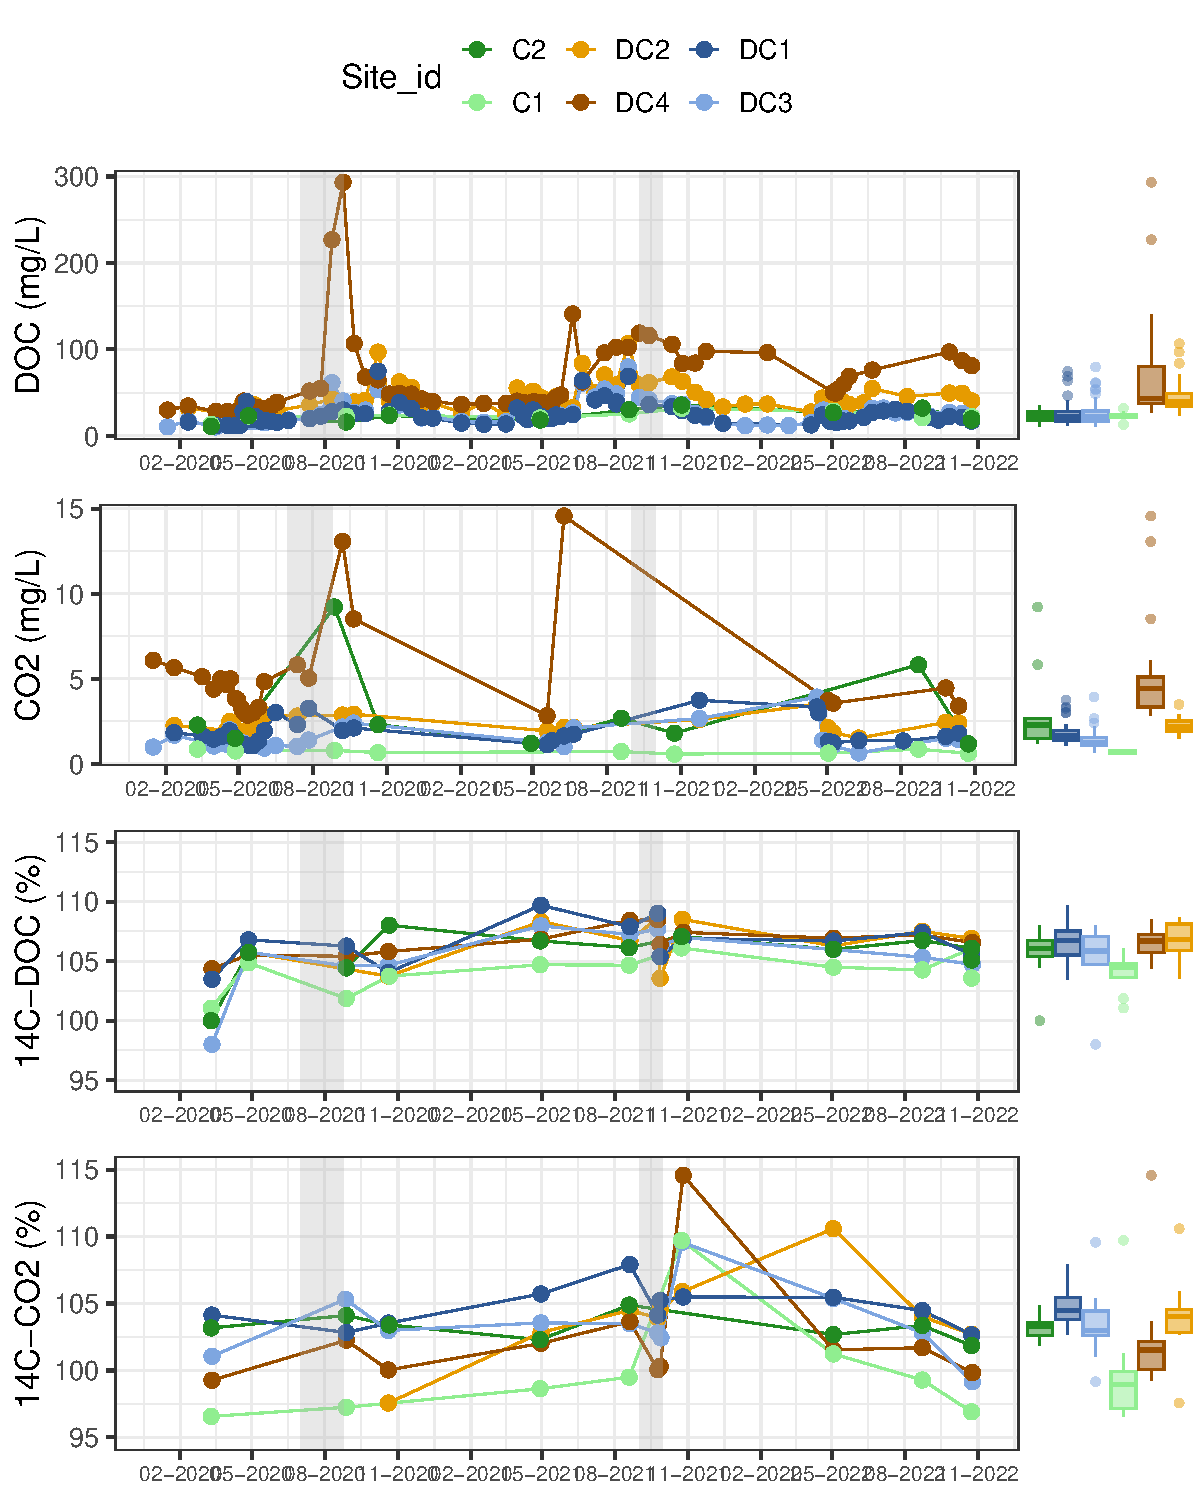
\includegraphics{index_files/figure-pdf/unnamed-chunk-3-1.pdf}

\paragraph{Dunn's test \textbar{} ¹⁴C and {[}C{]} \textasciitilde{}
Site}\label{dunns-test-uxb9ux2074c-and-c-site}

\begin{Shaded}
\begin{Highlighting}[]
\FunctionTok{library}\NormalTok{(dunn.test)}
\FunctionTok{library}\NormalTok{(multcompView)}
\FunctionTok{library}\NormalTok{(PMCMR)}
\CommentTok{\# Perform the test and get multcomp letters}
\NormalTok{DOCSites\_letters }\OtherTok{=} \FunctionTok{multcompLetters}\NormalTok{(}\FunctionTok{get.pvalues}\NormalTok{(PMCMRplus}\SpecialCharTok{::}\FunctionTok{kwAllPairsDunnTest}\NormalTok{(}
\NormalTok{          DC\_Q}\SpecialCharTok{$}\NormalTok{DOC\_mgL }\SpecialCharTok{\textasciitilde{}}\NormalTok{ DC\_Q}\SpecialCharTok{$}\NormalTok{Site\_id, }\AttributeTok{p.adjust=}\StringTok{"bonf"}\NormalTok{)),}
          \AttributeTok{threshold=}\FloatTok{0.05}\NormalTok{)}\SpecialCharTok{$}\NormalTok{Letters}

\NormalTok{DOC\_14C\_Sites\_letters }\OtherTok{=} \FunctionTok{multcompLetters}\NormalTok{(}\FunctionTok{get.pvalues}\NormalTok{(PMCMRplus}\SpecialCharTok{::}\FunctionTok{kwAllPairsDunnTest}\NormalTok{(}
\NormalTok{          DC\_Q}\SpecialCharTok{$}\NormalTok{DOC\_14C\_Modern }\SpecialCharTok{\textasciitilde{}}\NormalTok{ DC\_Q}\SpecialCharTok{$}\NormalTok{Site\_id, }\AttributeTok{p.adjust=}\StringTok{"bonf"}\NormalTok{)),}
          \AttributeTok{threshold=}\FloatTok{0.05}\NormalTok{)}\SpecialCharTok{$}\NormalTok{Letters}
        
\NormalTok{CO2Sites\_letters }\OtherTok{=} \FunctionTok{multcompLetters}\NormalTok{(}\FunctionTok{get.pvalues}\NormalTok{(PMCMRplus}\SpecialCharTok{::}\FunctionTok{kwAllPairsDunnTest}\NormalTok{(}
\NormalTok{          DC\_Q}\SpecialCharTok{$}\NormalTok{CO2\_mgL }\SpecialCharTok{\textasciitilde{}}\NormalTok{ DC\_Q}\SpecialCharTok{$}\NormalTok{Site\_id, }\AttributeTok{p.adjust=}\StringTok{"bonf"}\NormalTok{)),}
          \AttributeTok{threshold=}\FloatTok{0.05}\NormalTok{)}\SpecialCharTok{$}\NormalTok{Letters}

\NormalTok{CO2\_C14\_Sites\_letters }\OtherTok{=} \FunctionTok{multcompLetters}\NormalTok{(}\FunctionTok{get.pvalues}\NormalTok{(PMCMRplus}\SpecialCharTok{::}\FunctionTok{kwAllPairsDunnTest}\NormalTok{(}
\NormalTok{          DC\_Q}\SpecialCharTok{$}\NormalTok{CO2\_14C\_Modern }\SpecialCharTok{\textasciitilde{}}\NormalTok{ DC\_Q}\SpecialCharTok{$}\NormalTok{Site\_id, }\AttributeTok{p.adjust=}\StringTok{"bonf"}\NormalTok{)),}
          \AttributeTok{threshold=}\FloatTok{0.05}\NormalTok{)}\SpecialCharTok{$}\NormalTok{Letters}

        
\CommentTok{\# Combine into a data frame}
\NormalTok{combined\_dunns\_results }\OtherTok{\textless{}{-}} \FunctionTok{data.frame}\NormalTok{(}
  \AttributeTok{Site =} \FunctionTok{names}\NormalTok{(DOCSites\_letters),}
  \StringTok{"[DOC]"} \OtherTok{=} \FunctionTok{as.character}\NormalTok{(DOCSites\_letters),}
  \StringTok{"14C{-}DOC"} \OtherTok{=} \FunctionTok{as.character}\NormalTok{(DOC\_14C\_Sites\_letters),}
  \StringTok{"[CO2]"} \OtherTok{=} \FunctionTok{as.character}\NormalTok{(CO2Sites\_letters[}\FunctionTok{names}\NormalTok{(DOCSites\_letters)]),}
  \StringTok{"14C{-}CO2"} \OtherTok{=} \FunctionTok{as.character}\NormalTok{(CO2\_C14\_Sites\_letters[}\FunctionTok{names}\NormalTok{(DOCSites\_letters)]),}
  \AttributeTok{check.names =} \ConstantTok{FALSE}
\NormalTok{)}

\FunctionTok{print}\NormalTok{(combined\_dunns\_results)}
\end{Highlighting}
\end{Shaded}

\begin{verbatim}
  Site [DOC] 14C-DOC [CO2] 14C-CO2
1   C2     a      ab   abc     abc
2   C1     a       a     d       a
3  DC2     b       b     a      bc
4  DC4     b       b     b      ab
5  DC1     a       b    ac       c
6  DC3     a      ab    cd     abc
\end{verbatim}

\begin{tcolorbox}[enhanced jigsaw, opacitybacktitle=0.6, opacityback=0, arc=.35mm, left=2mm, toprule=.15mm, colback=white, coltitle=black, breakable, rightrule=.15mm, colbacktitle=quarto-callout-note-color!10!white, title=\textcolor{quarto-callout-note-color}{\faInfo}\hspace{0.5em}{Interpretation}, colframe=quarto-callout-note-color-frame, toptitle=1mm, bottomrule=.15mm, bottomtitle=1mm, titlerule=0mm, leftrule=.75mm]

There is no visible differences in the CO2 and DOC concentration and 14C
content trend over time.

The only noticeable effect was at DC4, where there was a clear peak in
DOC and CO2 concentration in the stream during clearcut opperations. CO2
and DOC concentration at this site is consistently higher than the other
sites.

\end{tcolorbox}

\begin{tcolorbox}[enhanced jigsaw, opacitybacktitle=0.6, opacityback=0, arc=.35mm, left=2mm, toprule=.15mm, colback=white, coltitle=black, breakable, rightrule=.15mm, colbacktitle=quarto-callout-important-color!10!white, title=\textcolor{quarto-callout-important-color}{\faExclamation}\hspace{0.5em}{Q data}, colframe=quarto-callout-important-color-frame, toptitle=1mm, bottomrule=.15mm, bottomtitle=1mm, titlerule=0mm, leftrule=.75mm]

The database contains DC3 and DC2 data, one ditch cleaned while the
other only clearcut. The C2 data is available but only compiled for the
14C point measurements.

\end{tcolorbox}

\subsection{Differences across
treatments}\label{differences-across-treatments}

Is there a significant change in the median \textsuperscript{14}C
content of CO\textsubscript{2} and DOC between sites or treatment based
on their distribution ?

\begin{Shaded}
\begin{Highlighting}[]
\CommentTok{\# Make a scatterplot to distinguish the grouping across sites}
\NormalTok{density\_14Cscatter\_sites }\OtherTok{=} 
\NormalTok{  ggExtra}\SpecialCharTok{::}\FunctionTok{ggMarginal}\NormalTok{(}
  
            \FunctionTok{ggplot}\NormalTok{(}\AttributeTok{data=}\NormalTok{DC\_Q,}
                 \FunctionTok{aes}\NormalTok{(}\AttributeTok{x=}\NormalTok{DOC\_mgL, }\AttributeTok{y=}\NormalTok{CO2\_mgL\_filled, }
                    \AttributeTok{color=}\NormalTok{Treatment))}\SpecialCharTok{+}
            \FunctionTok{stat\_density\_2d}\NormalTok{(}\FunctionTok{aes}\NormalTok{(}\AttributeTok{fill =}\NormalTok{ Treatment), }\AttributeTok{geom =} \StringTok{"polygon"}\NormalTok{, }\AttributeTok{linewidth=}\DecValTok{0}\NormalTok{,}
                             \AttributeTok{alpha =} \FloatTok{0.2}\NormalTok{)}\SpecialCharTok{+} 
            \FunctionTok{geom\_point}\NormalTok{(}\AttributeTok{size=}\DecValTok{1}\NormalTok{)}\SpecialCharTok{+}
            \FunctionTok{geom\_abline}\NormalTok{(}\AttributeTok{intercept=}\DecValTok{0}\NormalTok{,}\AttributeTok{slope=}\DecValTok{1}\NormalTok{, }\AttributeTok{linetype=}\StringTok{"dotted"}\NormalTok{)}\SpecialCharTok{+}
            \FunctionTok{scale\_color\_manual}\NormalTok{(}\AttributeTok{values=}\FunctionTok{c}\NormalTok{(treatments\_colors))}\SpecialCharTok{+}
            \FunctionTok{scale\_fill\_manual}\NormalTok{(}\AttributeTok{values=}\FunctionTok{c}\NormalTok{(treatments\_colors))}\SpecialCharTok{+}
            \FunctionTok{scale\_y\_log10}\NormalTok{()}\SpecialCharTok{+}
              \FunctionTok{scale\_x\_log10}\NormalTok{()}\SpecialCharTok{+}
            \FunctionTok{labs}\NormalTok{(}\AttributeTok{x=}\FunctionTok{bquote}\NormalTok{(}\StringTok{"DOC (mg L"}\SpecialCharTok{\^{}{-}}\DecValTok{1}\SpecialCharTok{*}\StringTok{")"}\NormalTok{), }
                   \AttributeTok{y=}\FunctionTok{bquote}\NormalTok{(}\StringTok{"CO"}\NormalTok{[}\DecValTok{2}\NormalTok{]}\SpecialCharTok{*} \StringTok{" (mg L"}\SpecialCharTok{\^{}{-}}\DecValTok{1}\SpecialCharTok{*}\StringTok{")"}\NormalTok{))}\SpecialCharTok{+}
              \FunctionTok{theme}\NormalTok{(}\AttributeTok{legend.position =} \StringTok{"none"}\NormalTok{), }
            \AttributeTok{type =} \StringTok{"boxplot"}\NormalTok{, }\AttributeTok{groupColour =} \ConstantTok{TRUE}\NormalTok{, }\AttributeTok{groupFill =} \ConstantTok{TRUE}\NormalTok{ ) }


\CommentTok{\# Make a scatterplot to distinguish the grouping across treatment}
\NormalTok{density\_14Cscatter\_treatment }\OtherTok{=} 
\NormalTok{ggExtra}\SpecialCharTok{::}\FunctionTok{ggMarginal}\NormalTok{(}
  
            \FunctionTok{ggplot}\NormalTok{(}\AttributeTok{data=}\NormalTok{DC\_Q,}\FunctionTok{aes}\NormalTok{(}\AttributeTok{x=}\NormalTok{DOC\_14C\_Modern, }\AttributeTok{y=}\NormalTok{CO2\_14C\_Modern, }
                    \AttributeTok{color=}\NormalTok{Treatment))}\SpecialCharTok{+}
               \FunctionTok{stat\_density\_2d}\NormalTok{(}\FunctionTok{aes}\NormalTok{(}\AttributeTok{fill =}\NormalTok{ Treatment), }\AttributeTok{geom =} \StringTok{"polygon"}\NormalTok{, }\AttributeTok{linewidth=}\DecValTok{0}\NormalTok{,}
                             \AttributeTok{alpha =} \FloatTok{0.2}\NormalTok{)}\SpecialCharTok{+} 
            \FunctionTok{geom\_point}\NormalTok{(}\AttributeTok{size=}\DecValTok{2}\NormalTok{)}\SpecialCharTok{+}
            \FunctionTok{geom\_abline}\NormalTok{(}\AttributeTok{intercept=}\DecValTok{0}\NormalTok{,}\AttributeTok{slope=}\DecValTok{1}\NormalTok{, }\AttributeTok{linetype=}\StringTok{"dotted"}\NormalTok{)}\SpecialCharTok{+}
            \FunctionTok{scale\_color\_manual}\NormalTok{(}\AttributeTok{values=}\FunctionTok{c}\NormalTok{(treatments\_colors))}\SpecialCharTok{+}
            \FunctionTok{scale\_fill\_manual}\NormalTok{(}\AttributeTok{values=}\FunctionTok{c}\NormalTok{(treatments\_colors))}\SpecialCharTok{+}
            \FunctionTok{scale\_y\_continuous}\NormalTok{(}\AttributeTok{limit=}\FunctionTok{c}\NormalTok{(}\DecValTok{95}\NormalTok{,}\DecValTok{115}\NormalTok{))}\SpecialCharTok{+}
            \FunctionTok{labs}\NormalTok{(}\AttributeTok{x=}\FunctionTok{bquote}\NormalTok{(}\StringTok{"∆"}\SpecialCharTok{\^{}}\DecValTok{14}\SpecialCharTok{*}\StringTok{"C{-}DOC (\% modern)"}\NormalTok{), }
                   \AttributeTok{y=}\FunctionTok{bquote}\NormalTok{(}\StringTok{"∆"}\SpecialCharTok{\^{}}\DecValTok{14}\SpecialCharTok{*}\StringTok{"C{-}CO"}\NormalTok{[}\DecValTok{2}\NormalTok{]}\SpecialCharTok{*}\StringTok{" (\% modern)"}\NormalTok{))}\SpecialCharTok{+}
              \FunctionTok{theme}\NormalTok{(}\AttributeTok{legend.position =} \StringTok{"bottom"}\NormalTok{), }
            \AttributeTok{type =} \StringTok{"boxplot"}\NormalTok{, }\AttributeTok{groupColour =} \ConstantTok{TRUE}\NormalTok{, }\AttributeTok{groupFill =} \ConstantTok{TRUE}\NormalTok{ )}
            


\FunctionTok{ggarrange}\NormalTok{(density\_14Cscatter\_sites,}
\NormalTok{density\_14Cscatter\_treatment, }\AttributeTok{nrow=}\DecValTok{2}\NormalTok{, }\AttributeTok{align=}\StringTok{"hv"}\NormalTok{)}
\end{Highlighting}
\end{Shaded}

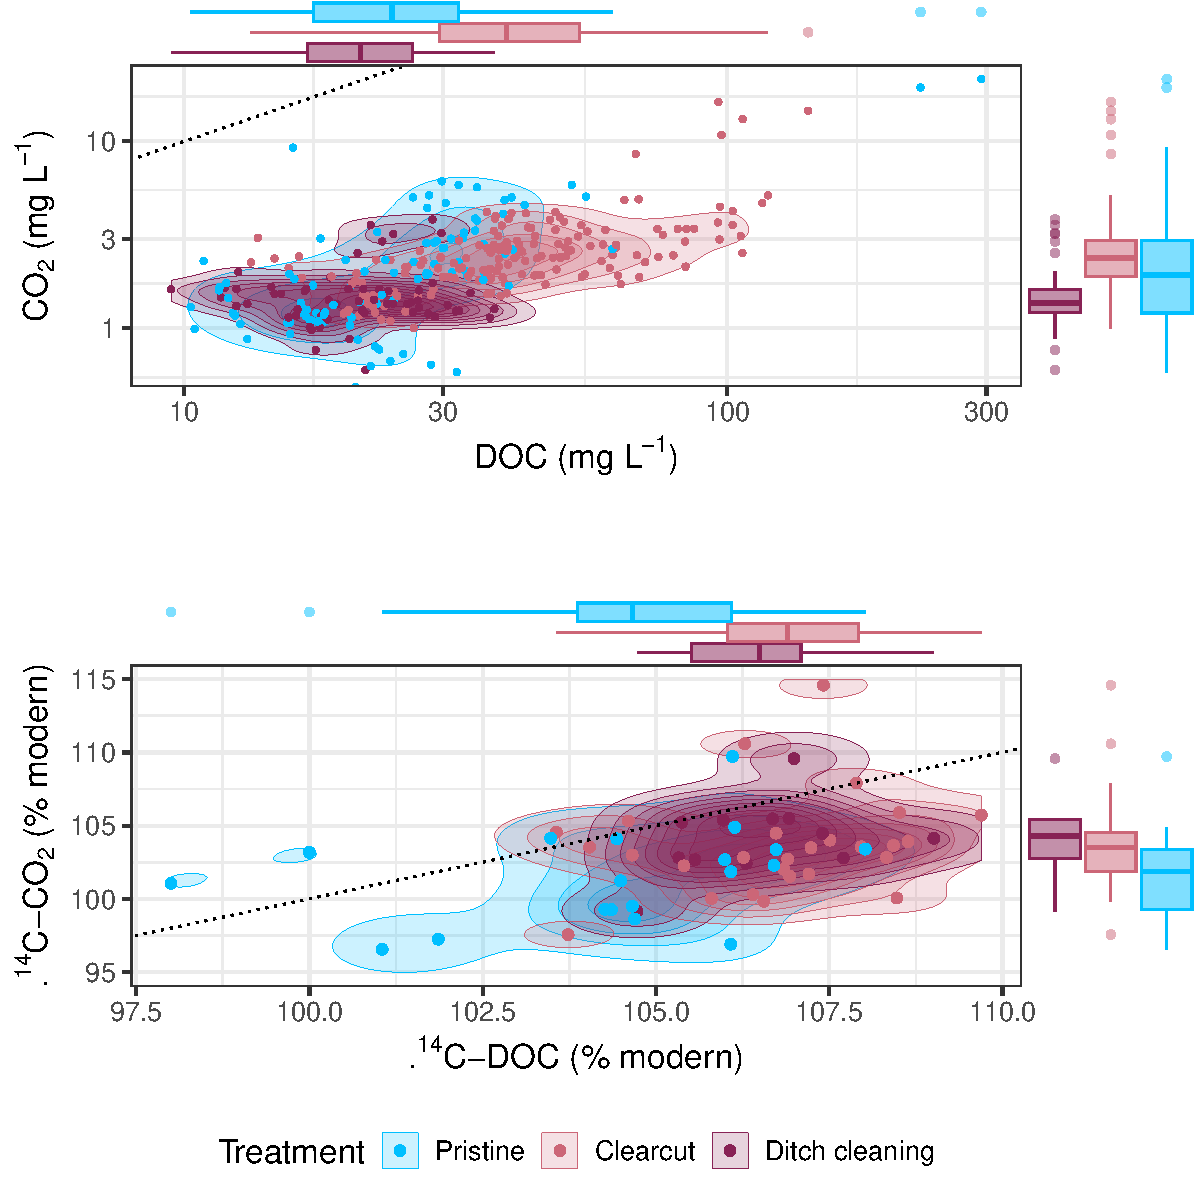
\includegraphics{index_files/figure-pdf/unnamed-chunk-5-1.pdf}

\paragraph{Dunn's test \textbar{} ¹⁴C et {[}C{]}\textasciitilde{}
Treatment}\label{dunns-test-uxb9ux2074c-et-c-treatment}

\begin{Shaded}
\begin{Highlighting}[]
\FunctionTok{library}\NormalTok{(dunn.test)}
\FunctionTok{library}\NormalTok{(multcompView)}
\FunctionTok{library}\NormalTok{(PMCMR)}

\CommentTok{\# Perform the test and get multcomp letters}
\NormalTok{DOCTreatment\_letters }\OtherTok{=} \FunctionTok{multcompLetters}\NormalTok{(}\FunctionTok{get.pvalues}\NormalTok{(PMCMRplus}\SpecialCharTok{::}\FunctionTok{kwAllPairsDunnTest}\NormalTok{(}
\NormalTok{          DC\_Q}\SpecialCharTok{$}\NormalTok{DOC\_mgL }\SpecialCharTok{\textasciitilde{}}\NormalTok{ DC\_Q}\SpecialCharTok{$}\NormalTok{Treatment, }\AttributeTok{p.adjust=}\StringTok{"bonf"}\NormalTok{)),}
          \AttributeTok{threshold=}\FloatTok{0.05}\NormalTok{)}\SpecialCharTok{$}\NormalTok{Letters}
        
\NormalTok{DOC\_C14\_Treatment\_letters }\OtherTok{=} \FunctionTok{multcompLetters}\NormalTok{(}\FunctionTok{get.pvalues}\NormalTok{(PMCMRplus}\SpecialCharTok{::}\FunctionTok{kwAllPairsDunnTest}\NormalTok{(}
\NormalTok{          DC\_Q}\SpecialCharTok{$}\NormalTok{DOC\_14C\_Modern }\SpecialCharTok{\textasciitilde{}}\NormalTok{ DC\_Q}\SpecialCharTok{$}\NormalTok{Treatment, }\AttributeTok{p.adjust=}\StringTok{"bonf"}\NormalTok{)),}
          \AttributeTok{threshold=}\FloatTok{0.05}\NormalTok{)}\SpecialCharTok{$}\NormalTok{Letters}
        
\NormalTok{CO2Treatment\_letters }\OtherTok{=} \FunctionTok{multcompLetters}\NormalTok{(}\FunctionTok{get.pvalues}\NormalTok{(PMCMRplus}\SpecialCharTok{::}\FunctionTok{kwAllPairsDunnTest}\NormalTok{(}
\NormalTok{          DC\_Q}\SpecialCharTok{$}\NormalTok{CO2\_mgL }\SpecialCharTok{\textasciitilde{}}\NormalTok{ DC\_Q}\SpecialCharTok{$}\NormalTok{Treatment, }\AttributeTok{p.adjust=}\StringTok{"bonf"}\NormalTok{)),}
          \AttributeTok{threshold=}\FloatTok{0.05}\NormalTok{)}\SpecialCharTok{$}\NormalTok{Letters}

\NormalTok{CO2\_C14\_Treatment\_letters }\OtherTok{=} \FunctionTok{multcompLetters}\NormalTok{(}\FunctionTok{get.pvalues}\NormalTok{(PMCMRplus}\SpecialCharTok{::}\FunctionTok{kwAllPairsDunnTest}\NormalTok{(}
\NormalTok{          DC\_Q}\SpecialCharTok{$}\NormalTok{CO2\_14C\_Modern }\SpecialCharTok{\textasciitilde{}}\NormalTok{ DC\_Q}\SpecialCharTok{$}\NormalTok{Treatment, }\AttributeTok{p.adjust=}\StringTok{"bonf"}\NormalTok{)),}
          \AttributeTok{threshold=}\FloatTok{0.05}\NormalTok{)}\SpecialCharTok{$}\NormalTok{Letters}

        
\CommentTok{\# Combine into a data frame}
\NormalTok{combined\_dunns\_results }\OtherTok{\textless{}{-}} \FunctionTok{data.frame}\NormalTok{(}
  \AttributeTok{Site =} \FunctionTok{names}\NormalTok{(DOC\_C14\_Treatment\_letters),}
  \StringTok{"14C{-}DOC"} \OtherTok{=} \FunctionTok{as.character}\NormalTok{(DOC\_C14\_Treatment\_letters),}
  \StringTok{"[DOC]"} \OtherTok{=} \FunctionTok{as.character}\NormalTok{(DOCTreatment\_letters),}
  \StringTok{"14C{-}CO2"} \OtherTok{=} \FunctionTok{as.character}\NormalTok{(CO2\_C14\_Treatment\_letters[}\FunctionTok{names}\NormalTok{(DOC\_C14\_Treatment\_letters)]),}
  \StringTok{"[CO2]"} \OtherTok{=} \FunctionTok{as.character}\NormalTok{(CO2Treatment\_letters[}\FunctionTok{names}\NormalTok{(DOC\_C14\_Treatment\_letters)]),}
  \AttributeTok{check.names =} \ConstantTok{FALSE}
\NormalTok{)}

\FunctionTok{print}\NormalTok{(combined\_dunns\_results)}
\end{Highlighting}
\end{Shaded}

\begin{verbatim}
            Site 14C-DOC [DOC] 14C-CO2 [CO2]
1       Pristine       a     a       a     a
2       Clearcut       b     b      ab     a
3 Ditch cleaning       b     a       b     a
\end{verbatim}

\begin{tcolorbox}[enhanced jigsaw, opacitybacktitle=0.6, opacityback=0, arc=.35mm, left=2mm, toprule=.15mm, colback=white, coltitle=black, breakable, rightrule=.15mm, colbacktitle=quarto-callout-note-color!10!white, title=\textcolor{quarto-callout-note-color}{\faInfo}\hspace{0.5em}{Interpretation}, colframe=quarto-callout-note-color-frame, toptitle=1mm, bottomrule=.15mm, bottomtitle=1mm, titlerule=0mm, leftrule=.75mm]

\textbf{Site effect}

\begin{itemize}
\item
  on \textsuperscript{14}C-DOC , differences more or less match
  treatment pairs (C1+C2, DC2+DC4, DC1+DC3), in three groups
\item
  on \textsuperscript{14}C-CO\textsubscript{2}, is significantly lower
  in DC4 and C1, 5 groups .
\end{itemize}

\textbf{Treatment} \textbf{effect}

\begin{itemize}
\item
  The \textsuperscript{14}C-DOC is significantly lower in the pristine
  (group a) compared with clearcut and ditch cleaning sites.
\item
  The \textsuperscript{14}C-CO\textsubscript{2} is significantly lower
  in the pristine compared with clearcut and ditch cleaning.
\end{itemize}

\end{tcolorbox}

\subsection{Relationships - controls on C sources, age and
concentrations}\label{relationships---controls-on-c-sources-age-and-concentrations}

\subsubsection{Hydrological control over C
concentrations}\label{hydrological-control-over-c-concentrations}

Is the radiocarbon age or concentration of DOC and CO\textsubscript{2}
controled by runoff, and does this relationship changes after treatment?

\begin{Shaded}
\begin{Highlighting}[]
\CommentTok{\# Hydrological control over  DOC concentration}
\NormalTok{hydro\_resp\_DOC}\OtherTok{=}
  \FunctionTok{ggplot}\NormalTok{(DC\_Q,}
       \FunctionTok{aes}\NormalTok{(}\AttributeTok{y=}\NormalTok{DOC\_mgL, }\AttributeTok{x=}\NormalTok{q\_md\_filled}\SpecialCharTok{*}\DecValTok{1000}\NormalTok{, }\AttributeTok{color=}\NormalTok{Site\_id))}\SpecialCharTok{+} 
  \FunctionTok{geom\_point}\NormalTok{(}\AttributeTok{size=}\DecValTok{1}\NormalTok{, }\AttributeTok{show.legend =}\NormalTok{ F)}\SpecialCharTok{+}
  \FunctionTok{scale\_x\_log10}\NormalTok{()}\SpecialCharTok{+}
  \FunctionTok{scale\_y\_log10}\NormalTok{()}\SpecialCharTok{+}
  \FunctionTok{geom\_smooth}\NormalTok{(}\AttributeTok{method=}\StringTok{"lm"}\NormalTok{, }\AttributeTok{se=}\NormalTok{F, }\FunctionTok{aes}\NormalTok{(}\AttributeTok{color=}\NormalTok{Site\_id), }\AttributeTok{show.legend =}\NormalTok{ T)}\SpecialCharTok{+}
  \FunctionTok{scale\_color\_manual}\NormalTok{(}\AttributeTok{values=}\NormalTok{site\_colors\_6)}\SpecialCharTok{+}
  \FunctionTok{stat\_regline\_equation}\NormalTok{(}\AttributeTok{label.y.npc =} \StringTok{"top"}\NormalTok{, }\AttributeTok{label.x.npc =} \StringTok{"left"}\NormalTok{,}
  \FunctionTok{aes}\NormalTok{(}\AttributeTok{label =}  \FunctionTok{paste}\NormalTok{(..eq.label.., ..adj.rr.label.., }
                     \AttributeTok{sep =} \StringTok{"\textasciitilde{}\textasciitilde{}\textasciitilde{}\textasciitilde{}"}\NormalTok{), }\AttributeTok{color =}\NormalTok{ Site\_id), }
                      \AttributeTok{show.legend =}\NormalTok{ F, }\AttributeTok{size=}\DecValTok{3}\NormalTok{)}\SpecialCharTok{+}
  \FunctionTok{labs}\NormalTok{(}\AttributeTok{x=}\StringTok{"q (mm/d)"}\NormalTok{, }
       \AttributeTok{y=}\FunctionTok{bquote}\NormalTok{(}\StringTok{"DOC (mg/L)"}\NormalTok{))}\SpecialCharTok{+}
  \FunctionTok{theme}\NormalTok{(}\AttributeTok{legend.position =} \StringTok{"top"}\NormalTok{, }\AttributeTok{base\_size=}\DecValTok{8}\NormalTok{)}




\CommentTok{\# Hydrological control over CO2 concentration}
\NormalTok{hydro\_resp\_CO2}\OtherTok{=}
  \FunctionTok{ggplot}\NormalTok{(DC\_Q,}
       \FunctionTok{aes}\NormalTok{(}\AttributeTok{y=}\NormalTok{CO2\_mgL, }\AttributeTok{x=}\NormalTok{q\_md\_filled}\SpecialCharTok{*}\DecValTok{1000}\NormalTok{, }\AttributeTok{color=}\NormalTok{Site\_id))}\SpecialCharTok{+} 
  \FunctionTok{geom\_point}\NormalTok{(}\AttributeTok{size=}\DecValTok{1}\NormalTok{, }\AttributeTok{show.legend =}\NormalTok{ F)}\SpecialCharTok{+}
  \FunctionTok{scale\_x\_log10}\NormalTok{()}\SpecialCharTok{+}
  \FunctionTok{scale\_y\_log10}\NormalTok{()}\SpecialCharTok{+}
  \FunctionTok{geom\_smooth}\NormalTok{(}\AttributeTok{method=}\StringTok{"lm"}\NormalTok{, }\AttributeTok{se=}\NormalTok{F, }\FunctionTok{aes}\NormalTok{(}\AttributeTok{color=}\NormalTok{Site\_id), }\AttributeTok{show.legend =}\NormalTok{ T)}\SpecialCharTok{+}
  \FunctionTok{scale\_color\_manual}\NormalTok{(}\AttributeTok{values=}\NormalTok{site\_colors\_6)}\SpecialCharTok{+} \CommentTok{\#"}
  
  \FunctionTok{stat\_regline\_equation}\NormalTok{(}\AttributeTok{label.y.npc =} \StringTok{"top"}\NormalTok{, }\AttributeTok{label.x.npc =} \StringTok{"left"}\NormalTok{,}
  \FunctionTok{aes}\NormalTok{(}\AttributeTok{label =}  \FunctionTok{paste}\NormalTok{(..eq.label.., ..adj.rr.label.., }
                     \AttributeTok{sep =} \StringTok{"\textasciitilde{}\textasciitilde{}\textasciitilde{}\textasciitilde{}"}\NormalTok{), }\AttributeTok{color =}\NormalTok{ Site\_id), }
                      \AttributeTok{show.legend =}\NormalTok{ F, }\AttributeTok{size=}\DecValTok{3}\NormalTok{)}\SpecialCharTok{+}
  \FunctionTok{labs}\NormalTok{(}\AttributeTok{x=}\StringTok{"q (mm/d)"}\NormalTok{, }
       \AttributeTok{y=}\FunctionTok{bquote}\NormalTok{(}\StringTok{"CO"}\NormalTok{[}\DecValTok{2}\NormalTok{]}\SpecialCharTok{*}\StringTok{" (mg/L)"}\NormalTok{))}\SpecialCharTok{+}
  \FunctionTok{theme}\NormalTok{(}\AttributeTok{legend.position =} \StringTok{"top"}\NormalTok{, }\AttributeTok{base\_size=}\DecValTok{8}\NormalTok{)}



\FunctionTok{ggarrange}\NormalTok{(hydro\_resp\_DOC, }
\NormalTok{          hydro\_resp\_CO2, }
          \AttributeTok{nrow=}\DecValTok{2}\NormalTok{, }\AttributeTok{common.legend =}\NormalTok{ T)}
\end{Highlighting}
\end{Shaded}

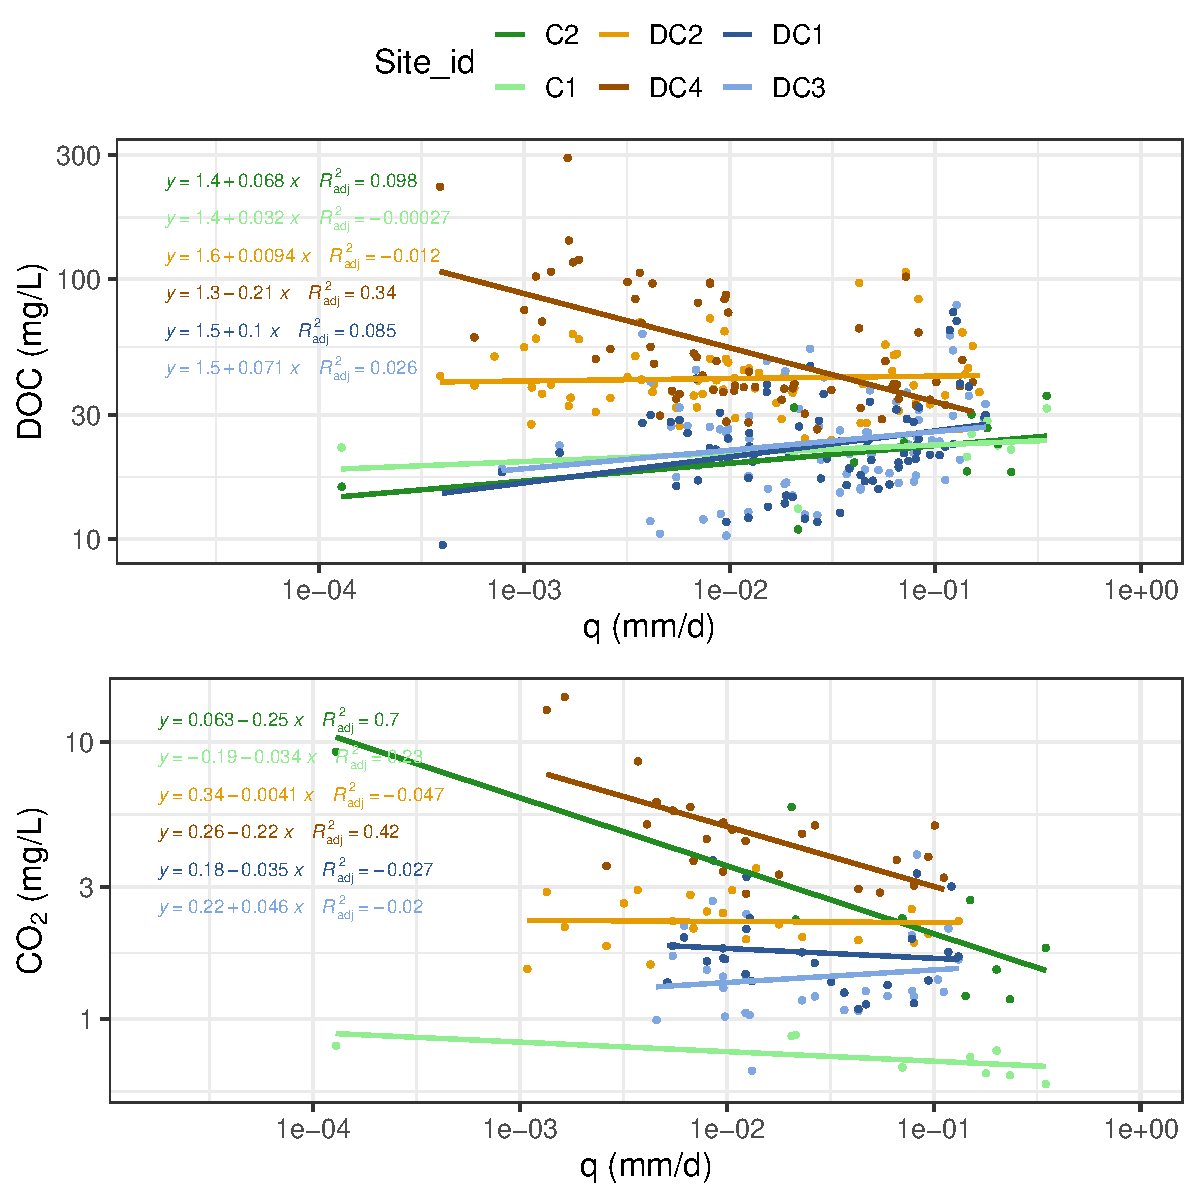
\includegraphics{index_files/figure-pdf/unnamed-chunk-7-1.pdf}

\begin{tcolorbox}[enhanced jigsaw, opacitybacktitle=0.6, opacityback=0, arc=.35mm, left=2mm, toprule=.15mm, colback=white, coltitle=black, breakable, rightrule=.15mm, colbacktitle=quarto-callout-note-color!10!white, title=\textcolor{quarto-callout-note-color}{\faInfo}\hspace{0.5em}{Interpretation}, colframe=quarto-callout-note-color-frame, toptitle=1mm, bottomrule=.15mm, bottomtitle=1mm, titlerule=0mm, leftrule=.75mm]

Carbon concentration in streams are mostly hydrology independant.

Relationships are significant, for :

\begin{itemize}
\item
  {[}DC4{]} DOC (negative) and CO2 (negative)
\item
  {[}C2{]} CO2 (negative), but not DOC.
\end{itemize}

\end{tcolorbox}

\subsubsection{\texorpdfstring{Hydrological controls over
\textsuperscript{14}C-content}{Hydrological controls over 14C-content}}\label{hydrological-controls-over-14c-content}

\begin{Shaded}
\begin{Highlighting}[]
\CommentTok{\#Scatter coloured by Treatment}
\FunctionTok{ggplot}\NormalTok{( DC\_Q }\SpecialCharTok{\%\textgreater{}\%} \FunctionTok{pivot\_longer}\NormalTok{(}
                     \AttributeTok{cols =} \FunctionTok{c}\NormalTok{(CO2\_14C\_Modern, DOC\_14C\_Modern),}
                     \AttributeTok{names\_to =} \StringTok{"Carbon\_specie"}\NormalTok{,}
                     \AttributeTok{values\_to =} \StringTok{"C14\_value"}
\NormalTok{                   ),}
       \FunctionTok{aes}\NormalTok{(}\AttributeTok{y=}\NormalTok{C14\_value, }\AttributeTok{x=}\NormalTok{q\_md\_filled}\SpecialCharTok{*}\DecValTok{1000}\NormalTok{, }\AttributeTok{fill=}\NormalTok{Treatment, }\AttributeTok{color=}\NormalTok{Treatment))}\SpecialCharTok{+}
  \FunctionTok{geom\_point}\NormalTok{(}\AttributeTok{size=}\DecValTok{3}\NormalTok{)}\SpecialCharTok{+}
  \FunctionTok{geom\_smooth}\NormalTok{(}\AttributeTok{method=}\StringTok{"glm"}\NormalTok{, }\AttributeTok{se=}\NormalTok{F, }\FunctionTok{aes}\NormalTok{(}\AttributeTok{color=}\NormalTok{Treatment), }\AttributeTok{show.legend =}\NormalTok{ F)}\SpecialCharTok{+}
  \FunctionTok{scale\_fill\_manual}\NormalTok{(}\AttributeTok{values=}\NormalTok{treatments\_colors)}\SpecialCharTok{+} 
  \FunctionTok{scale\_color\_manual}\NormalTok{(}\AttributeTok{values=}\NormalTok{treatments\_colors)}\SpecialCharTok{+} 
  
  \FunctionTok{stat\_regline\_equation}\NormalTok{(}
  \AttributeTok{label.y.npc =} \StringTok{"top"}\NormalTok{, }\AttributeTok{label.x.npc =} \StringTok{"left"}\NormalTok{,}
  \FunctionTok{aes}\NormalTok{(}\AttributeTok{label =}  \FunctionTok{paste}\NormalTok{(..eq.label.., ..adj.rr.label.., }
                     \AttributeTok{sep =} \StringTok{"\textasciitilde{}\textasciitilde{}\textasciitilde{}\textasciitilde{}"}\NormalTok{), }\AttributeTok{color =}\NormalTok{ Treatment), }
  \AttributeTok{show.legend =}\NormalTok{ F, }\AttributeTok{size=}\DecValTok{4}\NormalTok{)}\SpecialCharTok{+}
  \FunctionTok{labs}\NormalTok{(}\AttributeTok{x=}\StringTok{"q (m/d)"}\NormalTok{, }\AttributeTok{y=}\FunctionTok{bquote}\NormalTok{(}\StringTok{"∆"}\SpecialCharTok{\^{}}\DecValTok{14}\SpecialCharTok{*}\StringTok{"C (\% modern)"}\NormalTok{), }\AttributeTok{shape=}\StringTok{"Watershed ID"}\NormalTok{)}\SpecialCharTok{+}
  \FunctionTok{facet\_wrap}\NormalTok{(}\SpecialCharTok{\textasciitilde{}}\NormalTok{Carbon\_specie, }\AttributeTok{scale=}\StringTok{"fixed"}\NormalTok{, }\AttributeTok{nrow=}\DecValTok{1}\NormalTok{)}\SpecialCharTok{+}
  \FunctionTok{theme}\NormalTok{(}\AttributeTok{legend.position =} \StringTok{"top"}\NormalTok{)}
\end{Highlighting}
\end{Shaded}

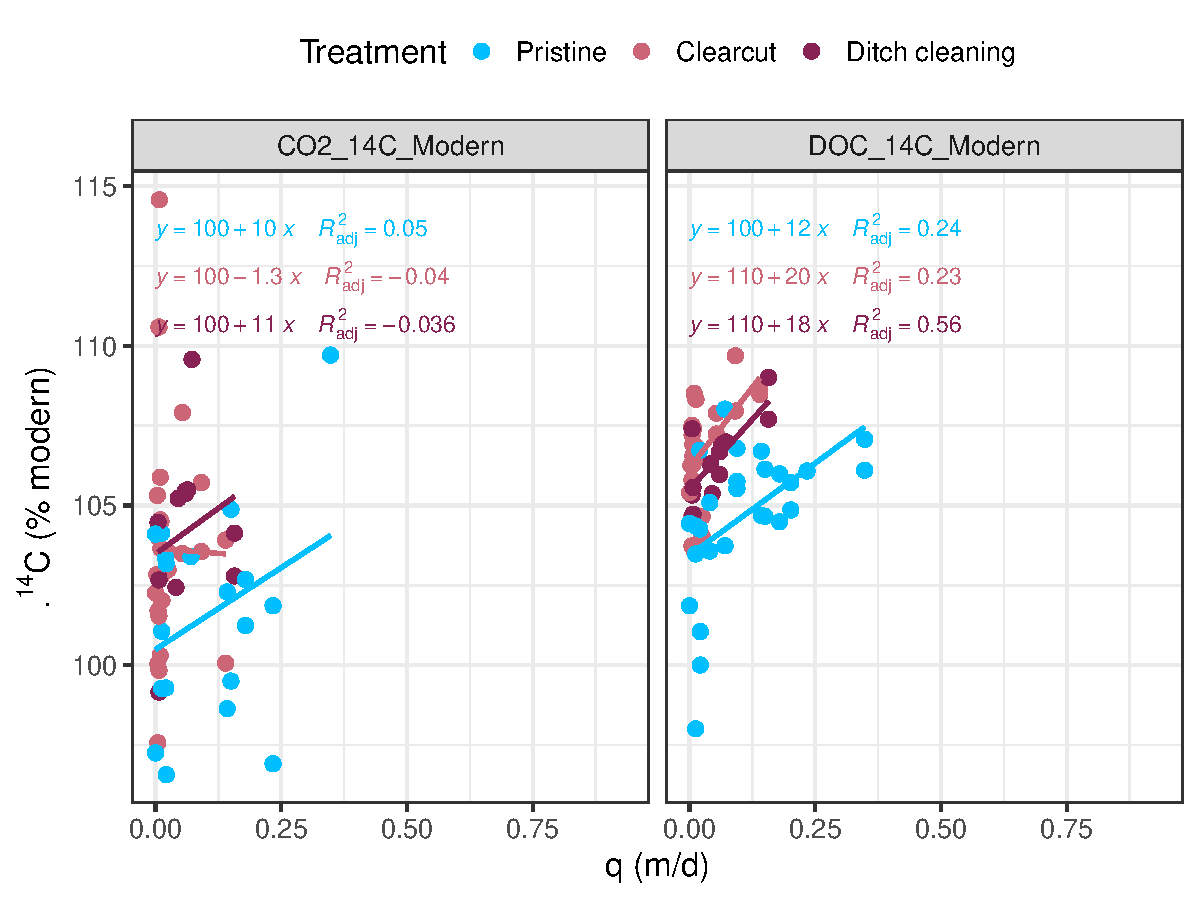
\includegraphics{index_files/figure-pdf/unnamed-chunk-8-1.pdf}

\paragraph{ANCOVA test}\label{ancova-test}

Is there a significant difference in the hydrological response of
\textbf{14C-DOC} between \emph{Treatments}?

\begin{verbatim}
ANOVA Table (type II tests)

                 Effect DFn DFd      F        p p<.05   ges
1           q_md_filled   1  62 24.164 6.81e-06     * 0.280
2             Treatment   2  62 22.767 3.86e-08     * 0.423
3 q_md_filled:Treatment   2  62  0.684 5.08e-01       0.022
\end{verbatim}

Is there a significant difference in the hydrological response of
\textbf{14C-CO2} between \emph{Treatments}?

\begin{verbatim}
ANOVA Table (type II tests)

                 Effect DFn DFd     F     p p<.05   ges
1           q_md_filled   1  52 1.816 0.184       0.034
2             Treatment   2  52 4.062 0.023     * 0.135
3 q_md_filled:Treatment   2  52 0.237 0.790       0.009
\end{verbatim}

\begin{Shaded}
\begin{Highlighting}[]
\CommentTok{\#Scatter coloured by sites}
\FunctionTok{ggplot}\NormalTok{( DC\_Q }\SpecialCharTok{\%\textgreater{}\%} \FunctionTok{pivot\_longer}\NormalTok{(}
                     \AttributeTok{cols =} \FunctionTok{c}\NormalTok{(CO2\_14C\_Modern, DOC\_14C\_Modern),}
                     \AttributeTok{names\_to =} \StringTok{"Carbon\_specie"}\NormalTok{,}
                     \AttributeTok{values\_to =} \StringTok{"C14\_value"}
\NormalTok{                   ),}
       \FunctionTok{aes}\NormalTok{(}\AttributeTok{y=}\NormalTok{C14\_value, }\AttributeTok{x=}\NormalTok{q\_md\_filled}\SpecialCharTok{*}\DecValTok{1000}\NormalTok{, }\AttributeTok{fill=}\NormalTok{Site\_id, }\AttributeTok{color=}\NormalTok{Site\_id))}\SpecialCharTok{+}
  \FunctionTok{geom\_point}\NormalTok{(}\AttributeTok{size=}\DecValTok{3}\NormalTok{)}\SpecialCharTok{+}
  \FunctionTok{geom\_smooth}\NormalTok{(}\AttributeTok{method=}\StringTok{"glm"}\NormalTok{, }\AttributeTok{se=}\NormalTok{F, }\FunctionTok{aes}\NormalTok{(}\AttributeTok{color=}\NormalTok{Site\_id), }\AttributeTok{show.legend =}\NormalTok{ F)}\SpecialCharTok{+}
  \FunctionTok{scale\_color\_manual}\NormalTok{(}\AttributeTok{values=}\NormalTok{site\_colors\_6)}\SpecialCharTok{+} 
  \FunctionTok{scale\_fill\_manual}\NormalTok{(}\AttributeTok{values=}\NormalTok{site\_colors\_6)}\SpecialCharTok{+} 
  \FunctionTok{stat\_regline\_equation}\NormalTok{(}
  \AttributeTok{label.y.npc =} \StringTok{"top"}\NormalTok{, }\AttributeTok{label.x.npc =} \StringTok{"left"}\NormalTok{,}
  \FunctionTok{aes}\NormalTok{(}\AttributeTok{label =}  \FunctionTok{paste}\NormalTok{(..eq.label.., ..adj.rr.label.., }
                     \AttributeTok{sep =} \StringTok{"\textasciitilde{}\textasciitilde{}\textasciitilde{}\textasciitilde{}"}\NormalTok{), }\AttributeTok{color =}\NormalTok{ Site\_id), }
  \AttributeTok{show.legend =}\NormalTok{ F, }\AttributeTok{size=}\DecValTok{4}\NormalTok{)}\SpecialCharTok{+}
  \FunctionTok{labs}\NormalTok{(}\AttributeTok{x=}\StringTok{"q (m/d)"}\NormalTok{, }\AttributeTok{y=}\FunctionTok{bquote}\NormalTok{(}\StringTok{"∆"}\SpecialCharTok{\^{}}\DecValTok{14}\SpecialCharTok{*}\StringTok{"C (\% modern)"}\NormalTok{), }\AttributeTok{shape=}\StringTok{"Watershed ID"}\NormalTok{)}\SpecialCharTok{+}
  \FunctionTok{facet\_wrap}\NormalTok{(}\SpecialCharTok{\textasciitilde{}}\NormalTok{Carbon\_specie, }\AttributeTok{scale=}\StringTok{"fixed"}\NormalTok{, }\AttributeTok{nrow=}\DecValTok{1}\NormalTok{)}\SpecialCharTok{+}
  \FunctionTok{theme}\NormalTok{(}\AttributeTok{legend.position =} \StringTok{"top"}\NormalTok{)}
\end{Highlighting}
\end{Shaded}

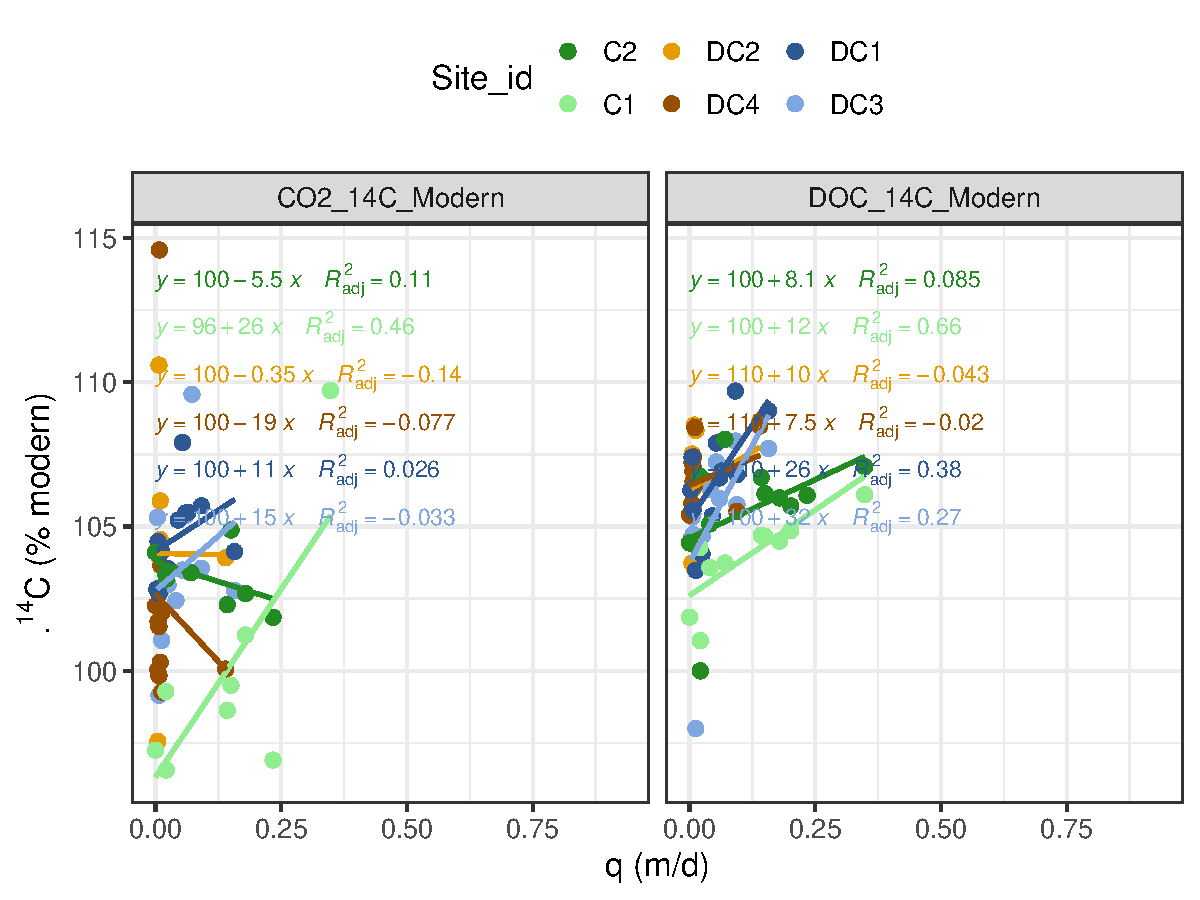
\includegraphics{index_files/figure-pdf/unnamed-chunk-11-1.pdf}

\paragraph{ANCOVA test}\label{ancova-test-1}

Is there a significant difference in the hydrological response of
\textbf{14C-DOC} between \emph{Sites}?

\begin{verbatim}
ANOVA Table (type II tests)

               Effect DFn DFd      F        p p<.05   ges
1         q_md_filled   1  56 18.570 6.68e-05     * 0.249
2             Site_id   5  56  6.873 4.60e-05     * 0.380
3 q_md_filled:Site_id   5  56  1.194 3.24e-01       0.096
\end{verbatim}

\begin{tcolorbox}[enhanced jigsaw, opacitybacktitle=0.6, opacityback=0, arc=.35mm, left=2mm, toprule=.15mm, colback=white, coltitle=black, breakable, rightrule=.15mm, colbacktitle=quarto-callout-note-color!10!white, title=\textcolor{quarto-callout-note-color}{\faInfo}\hspace{0.5em}{Interpretation}, colframe=quarto-callout-note-color-frame, toptitle=1mm, bottomrule=.15mm, bottomtitle=1mm, titlerule=0mm, leftrule=.75mm]

q has a significant effect on 14C-DOC, but not 14C-CO2

there is a significant effect of both Treatment and Sites in the model
(intercept differences), but no significant interaction (slope
differences).

The intercept shifts from 100\%modern in pristine sites, to 110\%modern
in clearcut+ditchcleaned sites.

\end{tcolorbox}

\paragraph{Linear mixed effect model}\label{linear-mixed-effect-model}

\begin{tcolorbox}[enhanced jigsaw, opacitybacktitle=0.6, opacityback=0, arc=.35mm, left=2mm, toprule=.15mm, colback=white, coltitle=black, breakable, rightrule=.15mm, colbacktitle=quarto-callout-note-color!10!white, title=\textcolor{quarto-callout-note-color}{\faInfo}\hspace{0.5em}{Interpretation}, colframe=quarto-callout-note-color-frame, toptitle=1mm, bottomrule=.15mm, bottomtitle=1mm, titlerule=0mm, leftrule=.75mm]

Make linear mixed effect model.

\end{tcolorbox}

\subsection{\texorpdfstring{Biological controls over
\textsuperscript{14}C-CO\textsubscript{2} - Keeling
plots}{Biological controls over 14C-CO2 - Keeling plots}}\label{biological-controls-over-14c-co2---keeling-plots}

\begin{Shaded}
\begin{Highlighting}[]
\NormalTok{DC\_Q}\SpecialCharTok{$}\NormalTok{CO2\_mgL\_filled\_keeling}\OtherTok{=} \DecValTok{1}\SpecialCharTok{/}\NormalTok{DC\_Q}\SpecialCharTok{$}\NormalTok{CO2\_mgL\_filled}
\NormalTok{DC\_Q}\SpecialCharTok{$}\NormalTok{CO2\_mgL\_filled\_keeling }\OtherTok{=} \FunctionTok{ifelse}\NormalTok{(}\FunctionTok{is.infinite}\NormalTok{ (DC\_Q}\SpecialCharTok{$}\NormalTok{CO2\_mgL\_filled\_keeling), }\ConstantTok{NA}\NormalTok{, DC\_Q}\SpecialCharTok{$}\NormalTok{CO2\_mgL\_filled\_keeling)}


\NormalTok{keeling}\OtherTok{=} \FunctionTok{ggplot}\NormalTok{(}\CommentTok{\#data = DC\_Q,}
\NormalTok{  DC\_Q }\SpecialCharTok{\%\textgreater{}\%} \FunctionTok{pivot\_longer}\NormalTok{(}
                     \AttributeTok{cols =} \FunctionTok{c}\NormalTok{(CO2\_14C\_Modern, d13C\_CO2),}
                     \AttributeTok{names\_to =} \StringTok{"Carbon\_isotope"}\NormalTok{,}
                     \AttributeTok{values\_to =} \StringTok{"isotope\_value"}
\NormalTok{                   ),}
       \FunctionTok{aes}\NormalTok{(}\AttributeTok{y=}\NormalTok{isotope\_value, }\AttributeTok{x=}\NormalTok{CO2\_mgL\_filled\_keeling, }
           \AttributeTok{color=}\NormalTok{Treatment))}\SpecialCharTok{+}
  
    \FunctionTok{geom\_smooth}\NormalTok{(}\AttributeTok{method=}\StringTok{"glm"}\NormalTok{, }\AttributeTok{se=}\NormalTok{F, }
                \AttributeTok{show.legend =}\NormalTok{ F)}\SpecialCharTok{+} 
    \FunctionTok{facet\_wrap}\NormalTok{(}\SpecialCharTok{\textasciitilde{}}\NormalTok{Carbon\_isotope, }\AttributeTok{scale=}\StringTok{"free"}\NormalTok{, }\AttributeTok{nrow=}\DecValTok{2}\NormalTok{)}\SpecialCharTok{+}
    \FunctionTok{stat\_regline\_equation}\NormalTok{(}
    \AttributeTok{label.y.npc =} \StringTok{"top"}\NormalTok{, }\AttributeTok{label.x.npc =} \StringTok{"left"}\NormalTok{, }\CommentTok{\#0.5}
    \FunctionTok{aes}\NormalTok{(}\AttributeTok{label =}  \FunctionTok{paste}\NormalTok{(..eq.label.., ..adj.rr.label.., }\AttributeTok{sep =} \StringTok{"\textasciitilde{}\textasciitilde{}\textasciitilde{}\textasciitilde{}"}\NormalTok{)), }\AttributeTok{show.legend =}\NormalTok{ F, }\AttributeTok{size=}\DecValTok{4}\NormalTok{)}\SpecialCharTok{+}
    
  \FunctionTok{geom\_point}\NormalTok{() }\SpecialCharTok{+}
  \FunctionTok{scale\_color\_manual}\NormalTok{(}\AttributeTok{values =}\NormalTok{ treatments\_colors) }\SpecialCharTok{+}
  \FunctionTok{scale\_fill\_manual}\NormalTok{(}\AttributeTok{values =}\NormalTok{ treatments\_colors) }\SpecialCharTok{+}
  \FunctionTok{theme}\NormalTok{(}\AttributeTok{legend.position =} \StringTok{"right"}\NormalTok{) }
  

\NormalTok{keeling}
\end{Highlighting}
\end{Shaded}

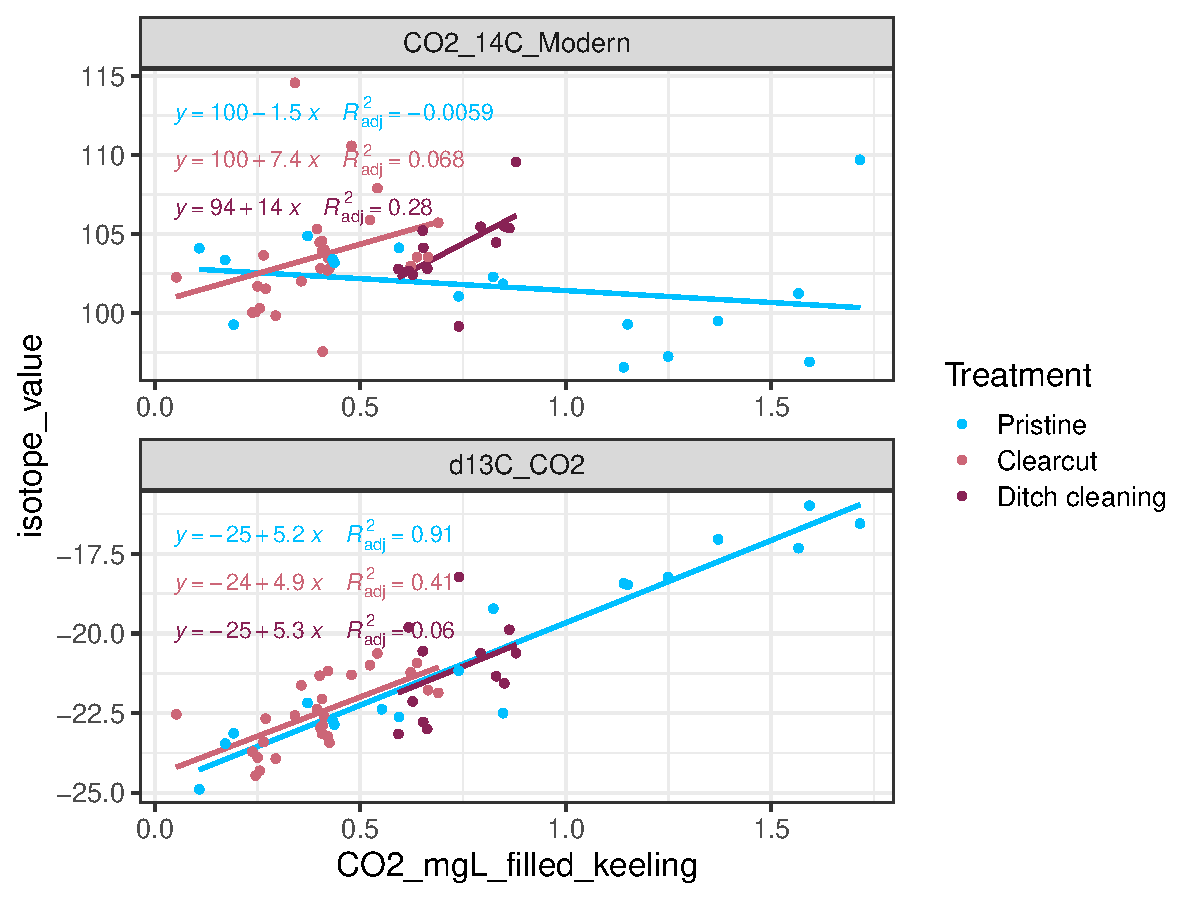
\includegraphics{index_files/figure-pdf/unnamed-chunk-14-1.pdf}

\begin{Shaded}
\begin{Highlighting}[]
\CommentTok{\#ggExtra::ggMarginal(keeling, }
\CommentTok{\#                    type = "boxplot", }
\CommentTok{\#                    groupColour = TRUE, }
\CommentTok{\#                    groupFill = TRUE,}
\CommentTok{\#                    alpha = 0.5)}
\end{Highlighting}
\end{Shaded}

\paragraph{ANCOVA test}\label{ancova-test-2}

Does the keeling for d13C-CO2 varies significantly between treatment or
sites?

\begin{Shaded}
\begin{Highlighting}[]
\CommentTok{\#Run ANCOVA test {-} Difference in hydro. response between Sites}
\NormalTok{DC\_Q }\SpecialCharTok{\%\textgreater{}\%} \FunctionTok{anova\_test}\NormalTok{(d13C\_CO2 }\SpecialCharTok{\textasciitilde{}}\NormalTok{ CO2\_mgL\_filled\_keeling}\SpecialCharTok{*}\NormalTok{Treatment)}
\end{Highlighting}
\end{Shaded}

\begin{verbatim}
ANOVA Table (type II tests)

                            Effect DFn DFd       F        p p<.05      ges
1           CO2_mgL_filled_keeling   1  51 145.233 1.53e-16     * 0.740000
2                        Treatment   2  51   0.527 5.93e-01       0.020000
3 CO2_mgL_filled_keeling:Treatment   2  51   0.018 9.83e-01       0.000687
\end{verbatim}

\begin{Shaded}
\begin{Highlighting}[]
\NormalTok{DC\_Q }\SpecialCharTok{\%\textgreater{}\%} \FunctionTok{anova\_test}\NormalTok{(d13C\_CO2 }\SpecialCharTok{\textasciitilde{}}\NormalTok{ CO2\_mgL\_filled\_keeling}\SpecialCharTok{*}\NormalTok{Site\_id)}
\end{Highlighting}
\end{Shaded}

\begin{verbatim}
ANOVA Table (type II tests)

                          Effect DFn DFd      F        p p<.05   ges
1         CO2_mgL_filled_keeling   1  45 20.763 3.96e-05     * 0.316
2                        Site_id   5  45  0.471 7.96e-01       0.050
3 CO2_mgL_filled_keeling:Site_id   5  45  0.515 7.63e-01       0.054
\end{verbatim}

Does the keeling for 14C-CO2 varies significantly between treatment or
sites?

\begin{Shaded}
\begin{Highlighting}[]
\CommentTok{\#Run ANCOVA test {-} Difference in hydro. response between Sites}
\NormalTok{DC\_Q }\SpecialCharTok{\%\textgreater{}\%} \FunctionTok{anova\_test}\NormalTok{(CO2\_14C\_Modern }\SpecialCharTok{\textasciitilde{}}\NormalTok{ CO2\_mgL\_filled\_keeling}\SpecialCharTok{*}\NormalTok{Treatment)}
\end{Highlighting}
\end{Shaded}

\begin{verbatim}
ANOVA Table (type II tests)

                            Effect DFn DFd     F     p p<.05      ges
1           CO2_mgL_filled_keeling   1  50 0.014 0.907       0.000277
2                        Treatment   2  50 2.409 0.100       0.088000
3 CO2_mgL_filled_keeling:Treatment   2  50 3.347 0.043     * 0.118000
\end{verbatim}

\begin{Shaded}
\begin{Highlighting}[]
\NormalTok{DC\_Q }\SpecialCharTok{\%\textgreater{}\%} \FunctionTok{anova\_test}\NormalTok{(CO2\_14C\_Modern }\SpecialCharTok{\textasciitilde{}}\NormalTok{ CO2\_mgL\_filled\_keeling}\SpecialCharTok{*}\NormalTok{Site\_id)}
\end{Highlighting}
\end{Shaded}

\begin{verbatim}
ANOVA Table (type II tests)

                          Effect DFn DFd     F     p p<.05   ges
1         CO2_mgL_filled_keeling   1  44 3.052 0.088       0.065
2                        Site_id   5  44 2.896 0.024     * 0.248
3 CO2_mgL_filled_keeling:Site_id   5  44 1.960 0.104       0.182
\end{verbatim}

\begin{tcolorbox}[enhanced jigsaw, opacitybacktitle=0.6, opacityback=0, arc=.35mm, left=2mm, toprule=.15mm, colback=white, coltitle=black, breakable, rightrule=.15mm, colbacktitle=quarto-callout-note-color!10!white, title=\textcolor{quarto-callout-note-color}{\faInfo}\hspace{0.5em}{Interpretation}, colframe=quarto-callout-note-color-frame, toptitle=1mm, bottomrule=.15mm, bottomtitle=1mm, titlerule=0mm, leftrule=.75mm]

The keeling plot suggests that the source of CO2 is the same across all
sites and treatments (-25‰) (no signficant effect of slope or intercept
across sites or treatment)

The 14C source, however, is not controled by CO2 concentration, but
still reveals a significant interaction between Treatment on the slope,
and site on the intercept. changes with treatments, from 100\%modern for
pristine and clearcut sites, but 94 for clearcut+ditchcleaned

\end{tcolorbox}

\phantomsection\label{refs}
\begin{CSLReferences}{1}{0}
\bibitem[\citeproctext]{ref-campeau2019}
Campeau, A., K. Bishop, N. Amvrosiadi, M. F. Billett, M. H. Garnett, H.
Laudon, M. G. Öquist, and M. B. Wallin. 2019. {``Current Forest Carbon
Fixation Fuels Stream CO2 Emissions.''} \emph{Nature Communications} 10
(1). \url{https://doi.org/10.1038/s41467-019-09922-3}.

\bibitem[\citeproctext]{ref-campeau2017}
Campeau, Audrey, Kevin H. Bishop, Michael F. Billett, Mark H. Garnett,
Hjalmar Laudon, Jason A. Leach, Mats B. Nilsson, Mats G. Öquist, and
Marcus B. Wallin. 2017. {``Aquatic Export of Young Dissolved and Gaseous
Carbon from a Pristine Boreal Fen: Implications for Peat Carbon Stock
Stability.''} \emph{Global Change Biology} 23 (12): 5523--36.
\url{https://doi.org/10.1111/gcb.13815}.

\bibitem[\citeproctext]{ref-ledesma2013}
Ledesma, J. L. J., T. Grabs, M. N. Futter, K. H. Bishop, H. Laudon, and
S. J. Köhler. 2013. {``Riparian Zone Control on Base Cation
Concentration in Boreal Streams.''} \emph{Biogeosciences} 10 (6):
3849--68. \url{https://doi.org/10.5194/bg-10-3849-2013}.

\bibitem[\citeproctext]{ref-uxf6quist2014}
Öquist, M. G., K. Bishop, A. Grelle, L. Klemedtsson, S. J. Köhler, H.
Laudon, A. Lindroth, M. Ottosson Löfvenius, M. B. Wallin, and M. B.
Nilsson. 2014. {``The Full Annual Carbon Balance of Boreal Forests Is
Highly Sensitive to Precipitation.''} \emph{Environmental Science \&
Technology Letters} 1 (7): 315--19.
\url{https://doi.org/10.1021/ez500169j}.

\end{CSLReferences}




\end{document}
